\chapter{Relay: A compiler framework for deep learning}
\label{ch:relay}

Relay is a collection of components for building a deep learning compiler, including optimizations, IR dialects, and system components.

Relay is designed in a middle-out style, by building in both a top-down, and bottom-up fashion we are able to design an IR which captures multiple frontends and backends, and provides clear semantics for program optimization.

Relay’s design was inspired by a set of guiding principles, the principle of least semantic, separation of concerns, and target independence.

The principle of least semantic dictates we should make design choices which give further optimization stages the ability to perform optimizations without unnecessary detail. For example enabling implicit effects and non-explicit control complicates computational graph semantics, and limits optimization. TF’s DAG attempts to separate pure semantics in order to handle out of order execution, and parallel and distributed scheduling, but does so by compromising on the programming model.

Instead we were able to build an IR inspired by the ML family of languages which provides pure-sub fragments which can be scheduled the same way without compromising on the programming model.

Another important semantic choice is that all Relay operators expose a functional interface, i.e they consume inputs and outputs. The functional semantics allow us to later introduce mutable buffers without requiring complex interprocedural program analysis.

Our second principle was a transparent separation from the abstract representation of machine learning models, and kernels. The abstraction is successfully introduced by computation graph IRs, but in an opaque way which limits cross layer optimization. Many gestalt approaches use a single language that defines all kernels and models, requiring users to both reason about all levels during optimization. We are able to represent abstract operations with well known types at the Relay level via the introduction of a user extensible shape dependent type system which can represent a wide range of operator’s types.

Our final guiding principle has been target independence. Relay was designed as a platform independent representation of machine learning computation. Given a known target, a user can schedule a new optimization, and all necessary platform optimizations and code generation will occur. Target independence might seem like a property already enjoyed widely, but in many frameworks each operator is implemented per platform, and often models only work on a single well-supported platform (i.e Nvidia GPU).  Previous IRs are either designed to be tethered to a specific end-user programming model or low-level operator library which enables the programs to be executed on specific platforms such as GPU.

Leveraging these features leads to powerful use cases, for example we are able to easily get best in class performance on many devices by mixing and matching TVM, with native kernel libraries to obtain the best performance, without the end user needing to adapt their program in anyway, see section N for more details.

There are many more examples we will cover in the next few sections of how Relay’s semantics enable novel solutions for domain-specific optimization. The rest of the section examines Relay’s design and properties which set it apart from previous solutions.

\section{Related Work}
\label{sec:related}

% TODO: We should be consistent in whether we use quotes or italics to
% introduce terms.

The acceleration of deep learning is an active topic of research and is
  cross-disciplinary by nature.
The dominant platforms for deep learning are TensorFlow, PyTorch, and MxNet.
Research on these frameworks cuts across all abstraction levels and
  involves experts from machine learning, systems, architecture, and programming languages (PL).
We first discuss the evolution of modern DL frameworks,
  then the lower-level components DL frameworks have incorporated to gain performance
  (i.e., low-level tensor compilers and DL compilers),
  and finally, we turn to approaches from the PL community.

\subsection{Deep Learning Frameworks}

In the early days of deep learning, practitioners and researchers would program
  in general-purpose languages like Python utilizing
  scientific computing libraries like NumPy,
  which provide low-level \textit{operators} such as matrix multiplication.
In order to accelerate model execution,
    frameworks supporting accelerators such as GPU were introduced~\cite{theano} .
Early frameworks represented models as directed ``computation graphs'',
    where each node represents an operator,
    and each edge represents the flow of data from one operator to another.
Computation graphs provide a limited programming model,
    enabling straightforward mapping of operators onto GPUs.
Large technology companies,
    such as Google, Facebook, and Amazon,
    drive the development of frameworks,
    and consequently,
    each company has its own stack consisting
    of the core framework (TensorFlow~\cite{tensorflow}, PyTorch~\cite{pytorch}, MxNet~\cite{mxnet}),
    compilers(XLA~\cite{xla}, Glow~\cite{glow}, TVM~\cite{tvm_osdi18}),
    and hardware accelerators (TPU~\cite{tpuv1}, GraphCore, Inferentia~\cite{inferentia}).
Frameworks can be roughly categorized into those which support \textit{static} computation graphs
  and those which support \textit{dynamic} computation graphs.
Frameworks which use static graphs are said to be \textit{define-and-run} frameworks,
  whereas frameworks which use dynamic graphs are said to be \textit{define-by-run} frameworks.

\subsection*{Define-And-Run Frameworks}

TensorFlow, Caffe~\cite{caffe}, and Theano~\cite{theano} are define-and-run frameworks.
Static graphs represent a whole-program,
  enabling optimization and simplified deployment,
  by removing the need for a host language like Python.
TensorFlow (TF) extends pure dataflow graphs with \textit{control edges}
      to emulate the functionality of \verb|if| and \verb|while|.
TF's representation captures many state-of-the-art models,
      provides support for heterogeneous hardware back-ends,
      and enables reverse-mode automatic differentiation~{\cite{ad_survey, tensorflow}}.
TF's encoding of control has limitations, as control-flow structures
    do not clearly map to familiar control-structures, instead using specialized
    encodings which make adapting traditional optimizations challenging.
Furthermore,
    unmodified TensorFlow does not support building models where the shape of
    the computation graph is dependent on the input,
    frustrating researchers who wish to experiment with complex models.
TensorFlow Fold addresses this \textit{particular} limitation~\cite{tensorflowfold}
    but offers no general and extensible solution.
% The encoding also requires \textit{ad hoc}, special-purpose operators such
%     as \verb|NextIteration| and the addition of special control edges to the graph.
The crux of the problem is the lack of generic mechanisms for users to
    define new control flow combinators (e.g., \verb|fold|) and data types.
% TensorFlow's programing model is relatively restricted and has led to a number
%     of solutions including TF Eager, AutoGraph, and JAX TODO CITE.
% Modifying frameworks in this manner is a considerable engineering effort
%     and does not scale.

\subsection*{Define-By-Run Frameworks}
PyTorch~\cite{pytorch_ad}, Gluon~\cite{gluon}, Chainer~\cite{chainer_learningsys2015},
    and TensorFlow eager-mode~\cite{tf_eager} are define-by-run frameworks which
    attempt to address the challenges of previous work.
The approach popularized by PyTorch is to use a host language (e.g., Python)
    to eagerly execute operations while simultaneously building a computation graph
    as a side effect.
By using the full host language,
  its features may be used to provide a highly expressive programming model to users.
However, dynamic frameworks construct a graph \textit{per program trace} and must re-optimize when
    the graph topology changes, costing CPU cycles and incurring communication overhead between the host
    machine and accelerators.
Instead of just representing traces, \relay combines the advantages of both worlds by
    representing the whole program ahead of time,
    while supporting constructs like control flow, first-class functions, and data structures.

\subsection{Low-Level Tensor Compilers}
Low-level tensor compilers are focused on the production
    of high-performance operators which implement compute-intensive
    operations such as matrix multiplication or convolution.
There are a number of competing approaches,
    both from academic and commercial entities, such as
    TVM~\cite{tvm_osdi18}, Halide~\cite{halide}, Tensor Comprehensions(TC)~\cite{tensor_comprehensions},
    and Diesel~\cite{diesel}.
The most notable designs are either inspired by the
    compute-schedule split introduced by Halide
    and adapted by TVM, or the polyhedral framework,
    as used by TC and Diesel.
% Early frameworks relied heavily on manually optimized operator libraries for GPUs (e.g., cuBLAS and cuDNN).
Operator compilers perform code generation for sets of scalar loop nests,
    but only represent a restricted subset of a whole program, ignoring details such as
    memory allocation/management, data structures, closures, and arbitrary control flow.
\relay focuses on composing generic operators, and the surrounding program
    into an efficiently orchestrated DL program.

\subsection{Deep Learning Compilers}

DL frameworks have adopted compilers
    to tackle both performance and portability
    for existing applications, most notably
    XLA~\cite{xla}, Glow~\cite{glow}, nGraph~\cite{ngraph}, ONNC~\cite{onnc},
    PlaidML~\cite{plaidml}, and ModelCompiler.
These \textit{graph compilers} use computation graph IRs and provide
    lowering onto a variety of targets.
Often graph compilers only perform high-level optimizations
    and then offload to vendor-specific libraries.
% % TODO(this point is dangling)
% In particular,
%     XLA has advanced support for the TPU,
%     and is focused on lowering static loop nests into efficient kernels.

Due to their limited programming model, they
    provide the same functionality as \relay with
    a more limited language.
The most comparable points to \relay are recent
    developments in the TensorFlow and PyTorch
    ecosystems of MLIR and TorchScript, respectively.
Google introduced MLIR as a path forward for
    unifying its myriad of IRs.
Upon first examination MLIR might appear to be
    a replacement for XLA and related TF compiler
    efforts, but it is not that.
MLIR is shared infrastructure for constructing
    a set of interoperating IR ``dialects'' which
    can be used to construct compilers.
The MLIR project is working on IR dialects
    for TF's IR and a low-level polyhedral IR,
    but does not yet have an end-to-end solution for
    deep learning built upon MLIR, the insights in
    this paper can guide MLIR's dialect development.

TorchScript is a high-level Python-like IR developed as the first
    layer of PyTorch's JIT compiler.
PyTorch (since v1.0) can rewrite a subset of user programs into
    TorchScript, an idealized subset of Python.
TorchScript can then be executed by the TorchScript VM or JIT-compiled to a target platform.
TorchScript sits many layers above code generation and must accommodate
    the flexible semantics of Python, which rules out entire classes of static analysis.
In order to optimize away this dynamic behavior, TorchScript has
    a profiling JIT mode which identifies stable program traces
    during execution.
These stable static traces can then be optimized by lower-level
    compilers such as Glow or \relay to perform the last level of code generation.
Microsoft released ModelCompiler, a system for efficiently compiling RNNs defined
    in CNTK to CPU.
ModelCompiler uses Halide to represent low-level operations, but lacks
    the expressivity of the \relay IR and only demonstrates support for CPUs.
% \TQC{The discussion in this paragraph was a bit long given the less importance of this compiler,
%   consider remove everything except for
%   the paragraph about expressivitity.
%   I think we can even safely remove this paragraph
%   and fold it to citations to ngraph etc. mention lack of expressivity.
%   It is a workshop paper of LearningSys 18 workshop
%   \url{http://learningsys.org/nips18/assets/papers/30CameraReadySubmissionmodelcompiler_camera_ready_no_final_flag.pdf}
% }
% \todo{Suggestion from OOPSLA reviewer A: ``Accelerating recurrent neural networks through
% compiler techniques and quantization,'' Li-Wen Chang et al., Workshop on Systems for
% ML, NeurIPS 2018.}
% ModelCompiler similarly uses Halide to represent low-level operations,
%     which provides fusion and other standard optimizations.
% Their high-level IR is not clearly described but appears to lack arbitrary
%     control-flow, first-class functions, or datatypes.
% They employ quantization but do not demonstrate how/if it can be extended,
%     or if low-bit (< 8) quantization is supported.
% They have shown support for CPU execution but provide no
%     story for GPUs or accelerators.

\subsection{Programming Languages for Deep Learning}
\label{sec:pl_techniques_in_dl}

% TODO ADD tensor type sytems cites
In recent years, the design of new programming languages,
    or the augmentation of existing ones, has become
    a popular area of research.
New languages designed for machine learning and related
    tasks include Lantern~\cite{lantern}, Lift~\cite{lift_lang}, Flux.jl~\cite{fluxjl}
    AutoGraph~\cite{moldovan2018autograph}, Swift for TensorFlow~\cite{tf_swift},
    and JAX~\cite{jax}.
Lantern \cite{lantern} is the most related work to \relay as it can
    be used as a code generator.
Lantern is a deep learning DSL in Scala
    that uses lightweight modular staging (LMS) to lower code into C++ and CUDA.
Lantern's defining feature is the use of delimited continuations to perform
    automatic differentiation.
Delimited continuations provide an elegant algorithm for AD,
    only requiring local transforms, but incurs cost of
    heap allocated structures, and a less straightforward
    mapping to define-by-run frameworks.
Lantern solves this problem by using a CPS transform which
    complicated further optimization and code generation.
Lantern does not yet support hardware accelerators, and
    does not focus on full program optimizations.
The alternative approach is the augmentation of languages to support deep learning,
  the most notable being systems like AutoGraph, Flux.jl, Swift for TensorFlow,
  and JAX.
These systems are designed to be user-facing programming
    environments for deep learning and use a compiler IR
    to generate code.
For all intents and purposes \relay could be the IR in
    question, therefore  \relay complements these systems well by
    providing a more expressive IR to map computation onto.

    \section{Related Work}
\label{sec:related}

% 2. Related work including a discussion of how your proposed work either
% leverages that work (e.g., techniques you plan to adopt) or differs from it
% (e.g., novel contributions).  For your generals report, we recommend you
% focus primarily on your work on Beacon for high-level frontends, Relay for IR
% design, and type-supported optimizations for diverse backend support.

In this section we will focus on related work, specifically deep learning
frameworks, IRs and compilers, low-level tensor code generation DSLs,
prior work on deep learning and programming languages, dynamic neural
networks, and hardware acceleration for deep learning.

\subsection{Background}

Deep learning (DL) has been used to achieve state-of-the-art results in
  applications ranging from computer vision to game
  playing to natural language processing.
Deep learning provides a collection of techniques for learning functions that are difficult
  to program directly.
A programmer solving a problem with DL performs three steps.
First, she specifies a parametric function (often called a \textit{model},
  \textit{neural network}, or simply \textit{network}) $F(\theta, x)$ of the function
  that computes the desired value.
She then \textit{trains} the model by applying an optimization algorithm to find a set of
  parameters $\theta$ that results in an acceptable approximation of the function on a
  collection of input-output pairs.
Finally, she uses her learned function to produce outputs for new inputs in
  a process called \textit{inference}.
While training and inference were once performed on the same machine,
  it is more common today to train models on a fleet of high-powered devices,
  since training is very computationally intensive.
The values learned from training can then be deployed for inference on less powerful systems,
  such as a single GPU, a mobile phone, or an FPGA.
This work is focused on helping a user wishing to utilize machine learning specify and optimize
  the neural networks they wish too with minimal fuss and maximal performance.

\paragraph{Deep Learning Frameworks}

In the past few years deep learning has become an essential
  piece of technology to large companies which rely heavily
  on machine learning powered services.
Technology companies such as Facebook and Google have large development
  teams dedicated to developing tools to support deep learning research
  and development.
Google is developing an ML stack comprised of
  TensorFlow, XLA, TPU, and a host of satellite projects.
Facebook is developing an ML stack comprised of
  many projects including PyTorch,
  Glow~\cite{glow}, and Caffe2~\cite{pytorch_caffe2}.
Amazon Web Services has been developing a stack
  comprised of many projects including
  MxNet, TVM, and Inferentia.

In the early days of deep learning, users would program
  in general purpose languages like Python and utilize
  scientific computing libraries like NumPy,
  which provides low-level \textit{operators} such as matrix multiplication.
Operators, also called kernels,
  are dense linear algebra primitives like matrix multiplication,
  elementwise functions like \verb|tanh|, and complex,
  domain-specific operations like image convolution.
Operator execution dominates the execution time of a deep learning model: many
  operators are asymptotically slow and their input is large.
While a machine learning framework may be written as a library in a high-level language
  like Python or Swift, operators will typically be provided as opaque function calls to
  specialized implementations written in a lower-level language like C++.

To obtain better performance, researchers began utilizing specialized
  accelerators such as GPUs to accelerate the execution of models.
In order to accessibly provide acceleration to end-users
  researchers designed frameworks like Theano~\cite{theano}.
Frameworks such as Theano and Torch introduced a model of
  computation graphs, dataflow graphs composed of nodes of
    variables, and operations on data.
These computation graphs represent the AST of a small
  embedded DSL that could be easily compiled and deployed
  to accelerators like the GPU.
``Computation graphs'' provide a limited programming model,
    enabling efficient deployment.
Computation graphs have since been adopted as the fundamental building block of modern
    machine learning libraries.

Unfortunately computation graphs are an ad-hoc language engineered to solve
  the problems faced at the time, and do not begin to capture the full breadth
  of models that users would one day want to run.
For example,
  convolutional neural networks (CNNs),
  which are widely used in image processing and computer vision,
  generally utilize a fixed topology of layers
  with tensors of fixed dimension.
In contrast,
  recurrent neural networks (RNNs),
  which are widely used in natural language processing (NLP),
  require recursion, control flow, and
  operations over variable-sized data structures (e.g., lists).
The regular structure of CNNs facilitates
  optimizing compilation to
  common hardware accelerators (e.g., GPUs), but
  RNN-like models are still challenging to optimize.

One area in which deep learning has made significant advances since
  the introduction of early frameworks is natural language processing (NLP).
Reasoning about text requires context-sensitive analysis and data of
    non-fixed dimensions, unlike in many vision tasks.
 To allow for context-sensitive analysis, DL researchers have developed networks with persistent
  state, known as \textit{recurrent neural networks}  (RNNs).
Recurrent neural networks have found use not only in NLP, but also in speech recognition, music
  transcription, eSports, and other areas \cite{lstm, speech_recognition, OpenAI_dota}.
Unfortunately, since most machine learning frameworks rely on computation graphs,
  which cannot directly represent recursion, RNNs are usually finitely unrolled to a fixed depth.
This is acceptable if the depth can be determined statically and the loop unrolled
  ahead of time; however, if the depth depends on runtime values or complex control flow,
  unrolling must be performed dynamically.

There are two dominant designs for computation graph-based frameworks.
The first is the declarative design employed by TensorFlow.
Such designs extend pure data-flow with \textit{ad hoc} control operations
  to emulate the functionality of \verb|if| and \verb|while|.
This approach is called \textit{define-then-run} and employs \textit{static
computation graphs}.
A framework using a define-then-run representation has access to the entire
  graph before execution, providing more opportunities to optimize the program
  as well as simplifying deployment since the program can be executed
  without the host language.
However, the control flow structures are less expressive than those supported
  by the host language, frustrating researchers who wish to experiment with complex models.
For example, TensorFlow supports loops,
  but the elaborated graph has little resemblance to the input program, requiring optimization
  authors to reason about the elaborated form instead of familiar loops.
The encoding also requires \textit{ad hoc}, special purpose operators such
  as \verb|NextIteration| and the addition of special control-edges to the graph.
There are no generic mechanisms for users to define new control flow
  combinators (e.g., \verb|fold|) or data types.
TensorFlow's representation is sufficient for many state-of-the-art models,
  is easily ported to heterogeneous hardware back-ends,
  and allows for reverse-mode automatic differentiation~{\cite{ad_survey, tensorflow}}.

The second approach is used by PyTorch, where the host language (e.g. Python) dynamically
  constructs a computation graph.
This approach is called \textit{define-by-run} and employs \textit{dynamic computation graphs}.
An arbitrary host program executes dynamically, generating a computation graph as a by-product,
  allowing for use of all host language features.
However, by not encoding control constructs in its IR, a framework
  using define-by-run cannot reason about or optimize control flow structures.
Not only does this leave performance on the table, but it prevents deployment to certain
  edge devices, since they may have control flow or memory requirements that cannot be
  guaranteed by a fully dynamic control plane.

Dynamic frameworks such as  PyTorch~\cite{pytorch_ad},
    Gluon~\cite{gluon},
    Chainer~\cite{chainer_learningsys2015},
    and TensorFlow eager-mode~\cite{tf_eager} are attempts to alleviate the
    challenges of static graph representations
These dynamic frameworks must re-optimize and rebuild as graph topology changes, costing
    CPU cycles and incurring communication overhead between the host machine and accelerators.
Relay is designed to solve many of the challenges with existing work, as
  discussed in Section \ref{sec:past}.

There is work from frameworks on trying to balance tradeoffs, most of which has
  been realized using advanced compilers.
There are a large number of deep learning compilers being
  developed today but have relatively similar designs.
The Glow compiler~\cite{glow} provides a graph-based IR designed for lowering
  to hardware accelerators.
XLA~\cite{xla}, within Google's TensorFlow, supports lowering statically sized
  loops nests down to existing vendor provided libraries or generating customized
  code platforms such as the Google TPU.
Intel's nGraph provides a similar graph-based IR, focused on representing DAGs
  of operations.
A serious challenge of these frameworks is the focus on a single layer of the
  stack, and restricted semantics, these challenges introduce the lack of
  flexibility discussed in Section \ref{sec:intro}.

\subsection{Hardware Backends}

Even if a model can execute on
  a particular hardware device, developers
  often manually design model
  variants for each target platform
  to achieve the best performance.
If a programmer wants to experiment with a new hardware device,
  she must manually account for variations in hardware intrinsics, data
  types, and data layout.
This is only possible if the device is supported by her framework of choice.
Even with the addition of device-specific code,
  there is no guarantee performance will be acceptable, let alone optimal
  (or even that there will not be regression).
Many existing IRs also do not support data-dependent control flow.
  platform's intrinsics and design.

Engineers design these platform specific model variants
  through tedious experimentation and framework-specific tweaks
  to achieve acceptable performance~\cite{mobilenet}. % xnor_net, squeezenet}.
For example,
  engineers may need to \textit{quantize} models
  by manually reducing numerical precision for a particular platform,
  sacrificing some accuracy for better performance~\cite{xnornet}.
Manually tuning models requires
  that engineers learn the details of
  each platform's
  unique data types, intrinsics, and memory systems~\cite{fb_fp_hw, tpuv1, brainwave, nn_on_si}.

The landscape of specialized hardware
  accelerators is also rapidly growing~\cite{
    moreau2018vta, OpenTPU, tpuv1}.
Accelerators provide an attractive way to decrease
  the execution time, memory and power consumption of models, as well
  as enable deep learning in new contexts.
Many deployment targets, such as mobile phones, are a heterogenous system
  consisting of a CPU, GPU, and customized machine learning accelerator.
Automatically targeting accelerators requires sophisticated compilers which
  must perform a variety of optimizations and schedule computation across
  heterogenous devices.
Hardware vendors need software stacks, often extending a deep learning
  compiler with support for their devices in the form of operations,
  optimizations, and datatypes.
It is essential that frameworks can adapt to new hardware devices
  with minimal changes to applications.
Relay provides an extensible framework for hardware accelerators,
  and implements a backend for \vta an emerging hardware accelerator\cite{moreau2018vta}.
We demonstrate how we can use an expressive general-purpose deep learning IR, plus
  a few platform specific optimizations

\subsection{High Performance DSLs for Tensors}

My work is focused on the end-to-end compilation of deep learning, and for
  this reason we do not directly focus on the generation of efficient low-level code for
  tensor operations.
Instead my work is focused on optimizing programs which make use of low-level operations
  and optimizations around programs which combine them with higher-level abstractions,
  like closures and datatypes.
In particular \relay is designed as an extension to \tvm~\cite{tvm_osdi18},
  a tensor expression language used for specifying dense array
  operations, to support full models.
Previous work on the \tvm focused on producing efficient operators
  (dense linear algebra kernels), such as generalized matrix multiplication (GEMM) and convolutions.
In theory \relay could use other high performance DSLs such as Halide~\cite{halide},
    which \tvm derived its IR, and its split computation and schedule model.
\todo{HALIDE EXPAND HERE}
Tensor Comprehensions (TC) shares common goals with the \tvm framework, but achieves its goal
through different techniques, such as polyhedral compilation rather than algorithmic
schedules. TC could replace \tvm in \relay{}'s compilation.
\todo{TC EXPAND HERE}

\subsection{Programming Language based Deep Learning}

My work is not the first attempt to apply programming language
    techniques to machine learning or problems such automatic differentiation.
\todo{LANTERN EXPAND}
Lantern \cite{lantern} is a deep learning DSL in Scala
    that uses lightweight modular staging (LMS) to lower code into C++.
LMS takes a graph as input from the user and converts it to an AST
    representation, similar to \relay's graph mode.
LMS removes unnecessary abstractions.
Going one step further than Lantern,
    \relay supports accelerators.

\verb|Flux.jl| \cite{fluxjl} is a DL library written in Julia \cite{julia}, a numerical
computing language. Like \relay, \verb|Flux.jl| adds shapes to the type system; however, unlike \relay, it
uses a mixture of compile-time inference and runtime checks to enforce shape constraints
\cite{jlmlpl} and cannot perform platform-specific optimizations. Unlike \verb|Flux.jl|, which
tightly coupled with Julia, \relay is language agnostic and decouples frontend and IR
considerations.
\relay's features, such as type inference and deployment to multiple back-ends, can
    be easily reused by frameworks in arbitrary languages.

Additionally, previous work in higher-order differentiation from the PL community
has informed \relay's design.
In particular, we draw inspiration from various implementations of
automatic differentiation \cite{beautiful_diff, ad_survey, haskell_ad, toplas_reverse, wang_reverse, DLS, DDF},
with particular attention to techniques that can compute higher-order gradients of higher-order programs.
\verb|Zygote.jl| \cite{zygotejl}, like \relay, uses source code transformations to
    implement automatic differentiation.

% end related

Frameworks for writing, compiling, and optimizing
  deep learning (DL) models have recently
  enabled progress in areas like computer
  vision and natural language processing.
Extending these frameworks to accommodate
  the rapidly diversifying landscape of
  DL models and hardware platforms presents
  challenging tradeoffs between
  expressivity, composability, and portability.
We present \relay,
  a new compiler framework for DL.
\relay's functional, statically typed intermediate representation (IR)
  unifies and generalizes existing DL IRs
  to express state-of-the-art models.
The introduction of \relay's expressive IR requires
  careful design of domain-specific optimizations,
  addressed via \relay's extension mechanisms.
Using these extension mechanisms,
  \relay supports a unified compiler that
  can target a variety of hardware platforms.
% \relay's extensible compiler
%   can eliminate abstraction overhead and
%   target new hardware platforms.
Our evaluation demonstrates \relay's competitive performance for a
  broad class of models and devices
  (CPUs, GPUs, and emerging accelerators).
\relay's design demonstrates how a unified IR can provide
  expressivity, composability, and portability
  without compromising performance.


Frameworks for writing, compiling, and optimizing
  deep learning (DL) models have recently
  enabled progress in areas like computer
  vision and natural language processing.
Extending these frameworks to accommodate
  the rapidly diversifying landscape of
  DL models and hardware platforms presents
  challenging tradeoffs between
  expressiveness, composability, and portability.
We present \relay,
  a new intermediate representation (IR)
  and compiler framework for DL models.
The functional, statically-typed \relay IR
  unifies and generalizes existing DL IRs
  and can express state-of-the-art models.
\relay's expressive IR required careful design of
  the type system, automatic differentiation, and optimizations.
\relay's extensible compiler
  can eliminate abstraction overhead and
  target new hardware platforms.
The design insights from \relay
  can be applied to existing frameworks
  to develop IRs that support extension
  without compromising on expressivity, composibility, and portability.
Our evaluation demonstrates that
  the \relay prototype can already provide
  competitive performance for a broad class of models
  running on CPUs, GPUs, and FPGAs.

%%   while retaining state
%%   of the art performance on a variety of targets.
%% Current frameworks use data-flow graphs as their only IR,
%%   restricting user programs, while
%% Popular DL frameworks internally represent models as dataflow graphs
%%   and provide idiosyncratic trade-offs between
%%   expressiveness, performance, and portability.
%% Current frameworks provide first class
%%   support for particular applications
%%   targeting a narrow range of hardware,
%%   and extending these frameworks is challenging.
%% This paper reports on \relay,
%%   a new functional, statically-typed intermediate representation (IR)
%%   for DL models.
%% \relay is designed to adapt to the rapidly changing world of deep learning,
%%   and support the demands of both researchers and engineers.
%% \relay unifies and generalizes existing deep learning IRs, leading
%%   to challenges in type checking, automatic differentiation, optimization,
%%   and compilation along the way.
%% As a result,
%%   \relay supports a broader class of applications than existing frameworks,
%%   unifies existing optimization approaches,
%%   and can target new hardware with minimal changes.
%% Our evaluation shows that \relay
%%   supports a broad class of models, incorporates optimization techniques
%%   from disparate tools, and provides competitive performance on
%%   CPUs, GPUs, and FPGAs all while being easy to extend.

  % - abstract needs to pop, more concrete

  % We present undergrad a new xxxx for
  % deep learning models.
  % Undergrad is more expressive,
  %   and more extensible then existing work while retaining state
  %   of the art performance on a variety of targets.
  % - current dlf use data-flow graph, restricting user programs,
  %   undergrad allows, a full programming paradigm
  % - Increasing the expressivity of undergrad incurs new challenges,
  %   namely how to adapt shape inference, and backprop, we can
  %   solve these problems by applying programming language techniques.
  % Hammer that is compiler framework, write opts, etc
  % The IR's expressiveness gives the \relay compiler implementation
  %   novel optimization opportunities exemplified by our generalize
  %   operator fusion, quantization framework, ....
  % Crucially \relay's design guarantees the composition of
  %   these optimizations even in the face of new operators,
  %   or new hardware backends.
  % LLVM HERE


  \section{Introduction}
  \label{sec:intro}

  Deep learning (DL) has radically transformed domains like
    computer vision and
    natural language processing (NLP)~\cite{yolo, recent_trends_in_nlp}.
  Inspired by these successes,
    researchers and companies are continually
    experimenting with increasingly sophisticated DL models and
    developing specialized hardware backends.
  DL frameworks for writing, optimizing, and compiling DL models
    reduce the complexity of these tasks,
    which in turn accelerates DL research and product development.

  Popular DL compiler intermediate representations (IRs) offer different tradeoffs
    between expressivity, composability, and portability~\cite{
      tensorflow, pytorch_ad, chainer_learningsys2015, tangent, theano, glow}.
  Early frameworks adopted IRs
    specialized for then-state-of-the-art models and/or
    emerging hardware accelerators.
  As a result, non-trivial extensions require
    patching or even forking frameworks~\cite{
      tf_fold, tf_lite, tangent, tf_eager, xla, glow, torchscript}.
  Such \textit{ad hoc} extensions can improve expressivity
    while maintaining backwards compatibility with existing execution mechanisms.
  However, they are difficult to design, reason about, and implement,
    often resulting in modifications that are mutually incompatible.

  Let us consider a hypothetical scenario that exemplifies
    IR design tensions in DL compilers.
  Suppose a machine learning engineer wants to write
    an Android app that uses sentiment analysis to
    determine the moods of its users.
  To maintain privacy, the app must run completely on-device,
    i.e., no work can be offloaded to the cloud.
  The engineer decides to use a variant of TreeLSTM,
    a deep learning model that uses a tree structure~\cite{tree_lstm}.
  Unfortunately, current frameworks' IRs cannot directly encode trees,
    so she must use a framework extension
    like TensorFlow Fold~\cite{tensorflowfold}.

%   Suppose that after adapting the model to run on her phone,
%     the out-of-the-box performance of her
%     model on her particular platform is not satisfactory, requiring her to optimize it.
%   She chooses to employ \textit{quantization}, an optimization that
%     potentially trades accuracy for performance by replacing
%     floating-point datatypes with low-precision ones.
%   Although researchers have developed a variety of quantization
%     strategies, each of which makes use of different bit-widths, rounding
%     modes, and datatypes, our engineer must use a strategy supported
%     by existing frameworks~\cite{gustafson2015end, tf_lite_ops_compat, glow_quant}.
  Unfortunately, frameworks only provide support for a small number
    of strategies, and supporting new quantization strategies is non-trivial.
  Each combination of operator, datatype, bit-width, and
    platform requires unique operator implementations.
  Optimizations like operator fusion exacerbate this combinatorial explosion,
    further increasing
    the number of unique implementations required.
  Furthermore, if a framework doesn't have specific support for
    the target phone model she cannot take advantage of specialized deep learning
    instructions or coprocessors~\cite{apple_neural_engine}.

  The scenario above highlights the three-pronged \textit{extensibility challenge}
    for DL IRs:
%   \begin{enumerate}[label=\arabic*.]
%     \item \textit{Expressivity}: It should be straightforward to write models involving
%       control flow, first-class functions and data structures (e.g., trees, graphs, and lists).
%     \item \textit{Composability}: It should be straightforward to add and compose new optimizations
%       with existing ones (e.g., quantization, operator fusion, and partial evaluation).
%     \item \textit{Portability}: It should be straightforward to add new hardware targets
%       (e.g., TPU, Inferentia)~\cite{tpuv1, inferentia}.
%   \end{enumerate}

  Previous IRs have struggled to address these challenges, treating each
    component of the framework as a disconnected set of programming tasks.
  Operators are defined in low-level languages like C++,
    connected by a dataflow graph, and then scripted
    in a host language like Python.
  Consequently,
    program analyses cannot cross language boundaries between components,
    inhibiting optimization and deployment.
  Learning from previous IRs, we have designed \relay,
    which features a principled approach to addressing extensibility
    and improves expressivity, composability, and portability
    over previous frameworks.
  We make the following contributions:
  \begin{itemize}
    \item The \relay IR, a tensor-oriented, statically typed
      functional IR,
      which we describe in Section \ref{sec:design}.
    \relay's design is motivated by the insight that functional IRs, used by
    languages from the ML family\footnote{``ML'' as in ``Meta Language,'' not
    ``Machine Learning''} can be readily adapted to support DL.
    With its \textit{expressive} semantics,
      including control flow, data structures, and first-class functions,
      \relay can represent entire state-of-the-art models.
    \item The insight that common features in ML frameworks,
      such as quantization and shape inference,
      can be reframed as standard compiler passes.
    By using this reframing we can tap into
      decades of traditional compilers research to design
      \textit{composable} optimization passes.
    \item
      A platform-agnostic representation of operators and domain specific
        optimizations which work in concert to provide \textit{portability}
        across hardware backends.
  \end{itemize}

  We evaluate \relay on several systems and over a diverse set of vision and NLP workloads to
    demonstrate that (1) \relay enables \emph{expressive} programs via a large breadth
    of models, (2) \relay supports \emph{composition} of program-level optimizations
    such as quantization and fusion, and (3) \relay provides
    \emph{portability} by targeting a number of hardware backends.
  Not only does \relay provide these three properties, we do so while also demonstrating
    competitive performance.
  \relay is an open-source academic project.\footnote{\relay is publicly available at [redacted for review].}
    It has been deployed at a popular web service provider,
      a telecommunications and consumer electronics manufacturer,
      and a social media company, among others.

      \section{Design}
      \label{sec:design}

      \relay's expressive high-level IR is designed to support
        complex models while abstracting over hardware-specific
        implementation details to enable hardware agnostic program
        analysis and optimization.
      Rather than invent an entirely new language,
        \relay's IR design is based on IRs used by the well-studied ML family of
        functional programming languages (e.g., SML and OCaml).
      These IRs are expressive enough to capture general-purpose programs
        (including control flow, first-class functions, and data types)
        and have clearly specified semantics (e.g., lexical scope and controlled effects).
      By borrowing from PL literature,
        we can apply program analysis and optimization techniques from decades of research~\cite{haskell_vector}.

      \relay's IR takes a small functional core and enriches it with domain-specific additions---namely,
        the inclusion of tensors and operators as expressions
        and a novel tensor type system design to support tensor shapes.
      Our principled design
        enables the import of existing models from deep learning frameworks and exchange formats,
        the implementation of a number of domain-specific optimizations,
        and efficient deployment across a variety of targets.
      In the remainder of this section,
        we describe the IR design in further detail
        and explore the ramifications of this design on the compilation stack.

      \subsection{IR}
      % \begin{figure}[!t]
%     \begin{jmpgrammar}
%       \bnfrule{REAL}{\real} \is{\mathbb{R}}\\
%       \bnfrule{NAT}{\nat} \is{\mathbb{N}}\\
%       \bnfrule{NAME}{\rName} \is{\texttt{(}\text{`\_'}\inlineAlt[a-zA-Z]\texttt{)}\ \
%       \atLeastZero{\text{`\_'}\inlineAlt[a-zA-Z]\inlineAlt[0-9]}}\\
%       \bnfrule{TYPE NAME}{\typename} \is{[A-Z]\ \ \atLeastZero{\text{`\_'}\inlineAlt[a-zA-Z]\inlineAlt[0-9]}}\\
%       \bnfrule{GLOBAL VAR}{\gvar} \is{\kwd{@}\rName}\\
%       \bnfrule{LOCAL VAR}{\lvar} \is{\kwd{\%} \rName}\\
%       \bnfrule{GRAPH VAR}{\graphVar} \is{\kwd{\%} \nat}\\
%       \bnfrule{TYPE VAR}{\tyvar} \is{\rName}\\
%       \bnfrule{OPERATOR}{\op} \is{\rName}\\\\
%       \bnfrule{Program}{\program} \is{\atLeastOne{\defn\inlineAlt\typedef}}
%         \alt{\expr}\\\\
%       \bnfrule{Param}{\param} \is{\rParamRule}\\
%       \bnfrule{Type Param}{\tyParam} \is{\rTyParamRule}\\\\
%       \bnfrule{Definition}{\defn} \is{\rDefnRule}\\\\
%       \bnfrule{Type Definition}{\typedef} \is{\rTypeDefRule}\\\\
%       \bnfrule{Kind}{\kind} \is{\kwd{BaseType}}
%         \alt{\kwd{Shape}}
%         \alt{\kwd{Relation}}
%         \alt{\kwd{ADT}}
%         \alt{\kwd{Type}}\\\\
%       \bnfrule{BaseType}{\basetype} \is{\kwd{int} \nat \maybe{\kwd{x} \nat}}
%         \alt{\kwd{float} \nat \maybe{\kwd{x} \nat}}
%         \alt{\kwd{bool} \maybe{\nat}}\\\\
%       \bnfrule{Shape}{\shape} \is{\kwd{(} \seq{\nat} \kwd{)}}\\\\
%       \bnfrule{Pattern}{\patt} \is[constructor]{\op \kwd{(} \seq{\patt} \kwd{)}}
%         \alt[wildcard]{\wildcard}
%         \alt[variable]{\lvar\ \maybe{\typeanno}}
%     \end{jmpgrammar}
%   \end{figure}
  \begin{figure}[t]
    % \ContinuedFloat
    \begin{jmpgrammar}
      \bnfrule{Expr}{\expr} \is[local var]{\lvar}
        \alt[global variable]{\gvar}
        \alt[constant tensor]{\kwd{const} \kwd{(} \texttt{(}\real\inlineAlt\bool\texttt{)} \kwd{,} \shape \kwd{,} \basetype \kwd{)}}
        \alt[call]{\expr \maybe{\tyargs} \args\vspace{0.2em}}
        \alt[let]{\rLetRule}
        \alt[\kwd{let}\ \kwd{\%}\_\ \kwd{=}\ \expr\kwd{;}\ \expr]{\rAnonLetRule}
        \alt[graph let]{\rGraphLetRule}
        \altSpace{0.5em}{function}{\rFnRule}
        % \altSpace{1em}{type cast?}{\kwd{(} \type \kwd{)} \expr}
        \altSpace{1em}{tuple formation}{\rTupRule}
        \alt[tuple proj.]{\rTupProjRule}
        \alt[if-else]{\rIfElse{\expr}{\expr}{\expr}}
        \altSpace{0.5em}{pattern match}{\rMatchRule}
        \altSpace{1em}{operator}{\op}
        % TODO: When will we have gradient as a first-class operator?
        % \alt[gradient]{\kwd{grad}\kwd{(}\expr\kwd{)}}
        \alt[new ref]{\kwd{ref}\kwd{(}\expr\kwd{)}}
        \alt[get ref]{\kwd{!} \expr}
        \alt[set ref]{\expr \kwd{:=} \expr}\\\\
      \bnfrule{Type}{\type} \is[base type]{\basetype}
        \alt[shape]{\shape}
        \alt[tensor type]{\kwd{Tensor} \kwd{[} \shape \kwd{,} \basetype \kwd{]}}
        \alt[type variable]{\tyvar}
        \alt[function type]{
          \begin{split}
          \kwd{fn}\ &\rTyParamsRule\\
          &\kwd{(} \seq{\type} \kwd{)}\ \rettype\\
          &\maybe{\relations}
          \end{split}
          }
        \alt[ref type]{\kwd{Ref} \kwd{[} \type \kwd{]}}
        \alt[tuple type]{\kwd{(} \seq{\type} \kwd{)}}
        \alt[type call]{\type \kwd{[} \seq{\type} \kwd{]}}
        \alt[type name]{\typename}
    \end{jmpgrammar}
    \caption{\textmd{The BNF Grammar for the \relay{} language.}}
    \label{fig:short_bnf}
  \end{figure}


      The \relay IR is designed
        to subsume the functionality of computation graph-based IRs
        while providing greater faculties for abstraction and control flow.
      We present \relay's design by incrementally building up to the full IR
        starting from a subset that corresponds to a simple computation graph.
      Deep learning models fundamentally operate on tensors.
      Hence, \relay's primary value type is a tensor and operators are included as language primitives
        (see the \verb|tensor constant| and \verb|operator| rules in Figure \ref{fig:short_bnf}).
      \relay leaves the implementation of each operator opaque; the operators
        are represented by a lower-level IR, which is optimized independently.
      A computation graph, in its simplest form, is a directed acyclic
        graph with multiple inputs and a single output.
      \relay uses three constructs to support these simple graphs:
        (1) \verb|variable|, (2) function \verb|call|,
        and (3) \verb|operator|; see Figure~\ref{fig:short_bnf} for the corresponding rules.

      \subsection*{Multiple Outputs}

      Computation graph IRs have primitive support for multiple outputs
        because many tensor operators require it.
      For example, the \verb|split| operator separates a tensor along a given axis
        and returns each component.
      In \relay, multiple outputs can be modeled as tuples,
        requiring only two rules: \verb|tuple formation| and \verb|tuple projection|.

      \subsection*{Let}

      By construction, computation graphs enjoy implicit sharing of subcomputations
        via multiple outgoing dependency edges.
      Implicit sharing is often implemented via pointers that uniquely identify subgraphs,
        a property useful for both execution and analysis.
      Previous frameworks often obtain this sharing by using a host
        language's name binding to construct a graph (e.g., by binding a Python variable
        to a subgraph and using that variable to construct other subgraphs).
      General-purpose programming languages, on the other hand, provide \textit{explicit}
        sharing via binding constructs, such as \verb|let|.
      In programs free of scope, ordering, and effects, implicit sharing
        and explicit sharing are semantically equivalent.
      However, in practice, user programs rely on effects and ordering,
        requiring previous approaches to provide workarounds.
      For example, TensorFlow's Eager Mode inserts dummy control edges
        in its generated graphs to impose effect ordering.
      The lack of lexical scope in computation graphs complicates language features,
        like first-class functions and control flow,
        and reduces the precision of traditional analyses,
        such as liveness,
        because the high-level program structure is absent~\cite{funarg, funarg_sol}.
      The addition of a humble \verb|let| binding, a central concept in functional languages,
        provides explicit sharing and a solution to the problems outlined above.

      \subsection*{Control Flow}

      \begin{figure*}[htb!]
        \begin{tabular}{ccc}
        \begin{minipage}{0.4\textwidth}
        \begin{minted}[fontsize=\small]{python}
      i = tf.constant(1)
      j = tf.constant(1)
      k = tf.constant(5)

      def c(i, j, k):
        return
          tf.equal(
            tf.not_equal(
              tf.less(i + j, 10),
              tf.less(j * k, 100)),
             tf.greater_equal(k, i + j))
      def b(i, j, k): return [i+j, j+k, k+1]
      tf.while_loop(c, b, loop_vars=[i, j, k])
        \end{minted}
        \end{minipage}
      & \hspace{-2.0em}
      \begin{Huge}
        $\Rightarrow$
      \end{Huge}
      &
        \begin{minipage}{0.5\textwidth}
        \begin{minted}[fontsize=\footnotesize]{python}
        fn %while_loop(
          %lvar0: Tensor[(1,), int32], %lvar1: Tensor[(1,), int32],
          %lvar2: Tensor[(1,), int32]) {
          %0 = add(%lvar0, %lvar1)
          %1 = less(%0, meta[Constant][0])
          %2 = multiply(%lvar1, %lvar2)
          %3 = less(%2, meta[Constant][1])
          %4 = not_equal(%1, %3)
          %5 = add(%lvar0, %lvar1)
          %6 = greater_equal(%lvar2, %5)
          if (min(equal(%4, %6))) {
            %9 = add(%lvar0, %lvar1)
            %10 = add(%lvar1, %lvar2)
            %11 = add(%lvar2, meta[Constant][2])
            %while_loop(%9, %10, %11)
          } else { (%lvar0, %lvar1, %lvar2)
          }
        }
        %while_loop(meta[Constant][3], meta[Constant][4], meta[Constant][5])
        \end{minted}
        \end{minipage}
        \end{tabular}
        \caption{\textmd{
          A simple TensorFlow loop in the user-facing DSL and the \relay
            loop produced by automatically converting it.
          Note the TensorFlow while loop corresponds neatly to a tail recursive
            function.
          The \relay text format supports a ``metadata'' section which functions
            as a constant pool among other things.
          \texttt{meta[Constant][n]} represents the \texttt{n}-th constant in the
            pool.
        }}
        \label{fig:tf_to_relay_loop}
        \end{figure*}

      Emerging models, particularly in the domain of natural language processing, increasingly
        rely on data-dependent control flow, forcing frameworks based on computation graph IRs
        to incorporate control flow, often through \textit{ad hoc} and difficult-to-extend constructs.
      For example, TensorFlow Fold~\cite{tf_fold} extends TF with special combinators that
        dynamically compute a graph for each shape permutation;
        these high-level constructs are opaque to further optimizations.
      The functional programming community has demonstrated that recursion and pattern matching are sufficient
        to implement arbitrary combinators for control flow and iteration (e.g., maps, folds, and scans).
      To support the definition of functional combinators
        we enrich \relay with two more language
        features to implement arbitrary combinators: \verb|if| and first-class recursive functions.

      \subsection*{First-Class Functions}

      A computation graph is a single computation
        from multiple inputs to multiple outputs.
      While it is tempting to reinterpret a graph as a function,
        graphs lack functional abstraction and named recursion.
      The addition of first-class named functions dramatically increases
        \relay's expressivity, allowing it to encode generic
        higher-order functions and thus capture higher-level program structure.
      First-class functions also enable simpler implementations
        of importers that map higher-level programs to our IR.
      For example, an instance of TensorFlow's looping construct \verb|tf.while_loop|
        can be represented as a single specialized loop function
        or a generic fold over the loop state.
      See Figure~\ref{fig:tf_to_relay_loop} for an example of this conversion (via
        the \relay TensorFlow frontend).

      \subsection*{Data Abstraction}
      Many models make use of additional data types beyond
        tuples, such as lists, trees, and graphs~\cite{char-rnn, tree_lstm, graph_lstm}.
      \relay borrows from functional languages
        a generic and principled method of extension:
        algebraic data types (ADTs).
      To support them, we add mechanisms for
        (1) type declaration and
        (2) pattern matching.
      This final addition results in a strict functional language,
        closely resembling the core of languages like OCaml and SML.
      The increase in expressivity introduced by the \relay IR introduces
        new optimizations challenges, which we
        discuss in Sec.~\ref{sec:optimizations}.

      \subsection{Type System}
      \label{subsec:type_system}

      \relay's type system is essential
        to optimizations.
      Typing guarantees both well-formedness of the program
        and provides crucial tensor shape information to perform allocation,
        check correctness, and facilitate loop optimizations.
      Shape information is also valuable for data layout transformations and tensorization,
        two transformations often demanded by hardware accelerators.
      In computation graph IRs, only numeric data types
        and shapes are tracked for each operator.
      Symbolic shapes (i.e., shape polymorphism) are only handled
        dynamically, inhibiting certain types of optimizations.

      It is possible to model arbitrarily complex static properties, such
        as shape information, with a dependent type theory~\cite{selsam_certigrad}, but such
        a design incurs significant user complexity.
      By incorporating shape analysis into a broader type system,
        \relay's type system balances the desire for static tensor shapes
        with usability.
      In this subsection, we describe how to extend a polymorphic type system with shape
        information and type inference with shape inference.

      \subsection*{Tensor Types}

      The primitive value in \relay is a tensor, which has
        a shape and a base type (\verb|tensor type| in Figure \ref{fig:short_bnf}).
      Base types describe the elements of tensors by tracking
        the bit width,
        the number of lanes (for utilizing vectorized intrinsics),
        and whether the type is floating point or integral.
      To ensure \relay can offload tensor computation to devices
        with greatly varying architectures,
        \relay tensors may only contain base types,
        preventing, for example, tensors of closures.
      The shape of a tensor is a tuple of integers describing the tensor's dimensions.
      A dimension may be a variable or arithmetic expression that indicates how the
        output shape of an operator depends on those of its inputs.
      Functions may be polymorphic over shapes, which results
        in shape constraints that must be solved during type inference.
      Sec.~\ref{sec:inference} describes the process.
      \relay also supports a special shape called \verb|Any|, which is used
        to mark a dynamic shape when static relationships are not profitable
        to model.

      \subsection*{Operators and Type Relations}
      Operators are one of the key primitives that differs from those of
        general-purpose programming languages.
      \relay's use of opaque operators enables backends to choose different
        lowering strategies based on the hardware target.
      \relay's operator set is extensible, meaning that users may add new operations.
      Supporting common or user-defined tensor operators requires a type system that can
        adapt to complex shape relationships between input and output types
        (e.g., elementwise operators with broadcasting semantics).

      To handle the constraints between operators' argument shapes, \relay's type system
        introduces type relations.
      A type relation is implemented as a function in the
        meta-language and represents a symbolic relationship between
        the input and output types.
      When developers add a new operator to \relay, they may constrain its
        type with an existing relation or add their own.
      Function types may include
        one or more type relations over a subset of the argument types and the return type.
      The type checker enforces that these relationships hold at each call site.

      \subsection*{Type Inference}
      \label{sec:inference}

      To incorporate type relations into \relay's type system, we enrich
        a Hindley-Milner-style type inference algorithm with
        a constraint solver.
      \relay's inference algorithm has three steps: first, it
        performs a pass over the AST, generating types and a set of relations,
        then it solves the incurred constraints,
        and finally annotates each sub-expression with its inferred type.

      % a queue of relations. dequeue a relation and attempt to solve it by invoking it's opaque
      % type-relation function.
      % 1. all type variables concrete & relationship holds => solved. discard relation
      % 2. all type variables concrete & relationship doesn't hold => type error
      % 3. types are partially symbolic => propagate unif. constraints to its inputs and output. if
      % all type variables are solved/assigned/concrete, discard relation. otherwise add it and the
      % relations that depend on the solved variables to queue. those that are already on the queue should
      % be reprioritized

      When the type inference algorithm visits a function call site, the function's type relations are
        instantiated with the concrete argument types at the call site.
      Each instantiated relation is added to the queue of relations to solve.
      The relationship between a call's type variables and relations is added as an edge to
        a bipartite dependency graph where the two disjoint sets are type variables and type relations.
      Traditional unification constraints are represented using a modified union-find structure that
        integrates with this dependency graph.

      Once the queue is populated, the algorithm will dequeue a relation and attempt to solve it.
      There are two cases when solving a type relation:
      \begin{enumerate}
        \item If all the relation's type variables
        are concrete, we the relation function. If that function returns true, the
        constraint is discharged. Otherwise, type checking fails.
        \item If any type is fully or partially symbolic, the
          algorithm will propagate
          existing concrete type information via unification.
        All relations affected by new assignments to type
          variables (as determined by the dependency graph)
          are moved to the beginning of the queue.
        If the current type relation is now completely solved, we
        discard it to avoid unnecessarily visiting it again.
      \end{enumerate}

      We run this to fixpoint or until the queue is empty.
      If the queue is non-empty and no progress is made between iterations,
        then at least one variable is underconstrained and inference fails.
      Note that a type relation's implementation can
        compromise type soundness, as they are axiomatic descriptions
        of operations implemented outside of \relay.
      In practice, the number of type relations needed to express \relay's
        operators is small, and their implementations are straightforward
        and amenable to exhaustive testing.

      \subsection{Compiler Framework}

      The process for compiling \relay proceeds in three stages.
      First, the frontend converts input formats into the \relay IR.
      Next, the \relay compiler typechecks and optimizes the program
        to produce the final program.
      After performing optimizations,
        the \relay backend transforms
        the \relay program into a form that can be executed on
        the intended hardware, based on the specified execution mechanism.
      The backend additionally lowers \relay operators into a TVM expression,
        computes a schedule for the final TVM expression, and lowers it into
        native code.

      \subsection*{Frontend}

      There are several ways to write an \relay program.
      A user can build an in-memory representation of
        a program in C++ or Python,
        parse one written in the \relay text format,
        load one from the on-disk serialization format,
        or import one from popular frameworks and interchange formats
          (e.g., TensorFlow, MxNet, Keras, DarkNet, and ONNX).
      Many frameworks and interchange formats use static computation graph-based representations,
        which can easily be translated into \relay.
      A greater challenge is translating frameworks
        with a richer computation model such as TensorFlow (TF).
      TF supports control flow and includes \verb|TensorArray|, a write-once
        tensor container.
      We can extract the loop structure out of the TF graph, converting
        it to an \relay loop, and transform the \verb|TensorArray| into an \relay list.
      Once new deep learning languages and IRs under development
        are stable it is likely they can be translated into \relay (see
        Section~\ref{sec:pl_techniques_in_dl}).
      PyTorch provides an expressive programming model, and is a good fit
        for \relay, which has integration into PyTorch's JIT infrastructure,
        enabling users to transparently use \relay for improved performance.

      \subsection*{Compiler}
      Once an \relay abstract syntax tree (AST) is produced,
        the program is optimized by applying a series of \relay-to-\relay
        passes.
      Between each pass, \relay performs type inference and checking,
        rejecting malformed programs as well as populating shape and type
        information that passes can utilize.
      The \relay compiler supports traditional optimizations
        (e.g., constant folding, common subexpression elimination, and dead code elimination)
        and domain-specific optimizations
        (see Sec.~\ref{sec:optimizations}).

      \subsection*{Backends}

      \relay produces machine-specific code
        by decomposing the problem of code generation into multiple distinct phases.
      \relay translates all operators into \tvm expressions
        to produce dense linear algebra kernels~\cite{tvm_osdi18, tensor_comprehensions, halide}.
      \tvm produces low-level operators that expect a fixed calling convention,
        as well as preallocated inputs and outputs.
      The result is an object file containing hardware-specific implementations of all
        operations.
      The remaining \relay program then is executed or compiled,
        with operator invocations replaced by calls to the optimized operators.
      By representing operators as \tvm expressions, we can programmatically
        transform them and automatically generate new implementations for the transformed operators.
      Optimizations like fusion and quantization
        rely on this novel behavior.
      After primitive operators are lowered,
        the remaining \relay program ties
        together operator invocations, allocation, control-flow,
        recursion, and high-level data structures.
      There are multiple options for executing the combined full program:
        the \relay interpreter (with JIT compilation),
        an \relay virtual machine,
        the \tvm graph runtime,
        and an experimental \relay ahead-of-time compiler
        that converts programs to C++ to produce a target-specific binary.
      % We are able to target CPU, GPU,
      %   iOS and Android mobile devices,
      %   custom accelerators, and FPGAs.


      % EVAL
      \section{Evaluation}
\label{sec:eval}

% 5. Methodology and evaluation: how do you plan to evaluate whether your ideas
% work or your hypotheses are correct?

In my proposal I make three specific claims we must evaluate,
\textbf{To develop an intelligent (1) end-to-end deep learning compiler that can
automatically adapt (2) high-level programs to run on new hardware devices automatically
with (3) human level performance.}

We evaluated \relay on several systems (x86 CPUs, ARM CPUs, NVIDIA GPUs, Xilinx FPGAs) and over
  diverse vision and NLP workloads to demonstrate that (1) \relay enables \emph{composability} of
  graph-level optimizations, (2) \relay delivers \emph{performance} on inference tasks competitive
  with state-of-the-art frameworks (TensorFlow, PyTorch, MxNet), and (3) \relay provides
  \emph{portability} over difficult-to-compile-to hardware backends such as FPGAs

\subsection{Relay: A high-level IR for Deep Learning}
  In particular, our evaluation is composed of three parts:
  \begin{enumerate}
    \item \textbf{\relay enables composable optimizations}: \relay
      supports composing program transformations into multiple optimization tiers.
    \item \textbf{\relay provides competitive performance}: Despite increasing
      expressiveness, \relay's performance is competitive with the
      state of the art on popular models.
    \item \textbf{\relay handles challenging backends}: \relay can compile
      models to execute efficiently on a variety of
      backends, such as FPGA accelerators, which require quantization, layout
      optimizations, and bit-packing transformations.
    % \item \textbf{\relay supports expressive models}: It can compile models with complex control flow
    % like Char-RNN to a single lean binary, beating PyTorch inference performance by up to 3x.
  \end{enumerate}

  We evaluated the following vision models:
    \textit{Deep Q-Network (DQN)}, a DNN that achieved state-of-the-art performance
    on 49 Atari games in 2015;
    \textit{MobileNet}, a DNN designed for image recognition on mobile and
    embedded devices;
    \textit{ResNet-18}, a DNN for image recognition that achieved state-of-the-art
    performance on ImageNet detection tasks in 2015;
    \textit{VGG-16} (named for the Visual Geometry Group
    at Oxford), a CNN used for image recognition tasks
    \cite{dqn, mobilenet, resnet, vgg}.

  We evaluated the following NLP models:
    \textit{CharRNN}, a generator character-level
    RNN from a PyTorch tutorial;
    \textit{TreeLSTM}, a generalization of LSTMs to
    tree-structured network topologies;
    \textit{RNN, GRU, and LSTM}, a selection of models from the Gluon
    model zoo
    \cite{pytorch_rnn_tut, tree_lstm, gluon_model_zoo}.

  \subsection{Experimental Methodology}
  % Because we only evaluate inference in this paper,
  %   we frequently make use of random inputs to models when measuring
  %   performance.
  % There were two exceptions where we evaluated on real data because
  %   it was readily available: CharRNN and TreeLSTM.

  % % For models where the input is random,
  % %   we run 1000 timed iterations.
  % % Before the timed runs,
  % %   we run 8 untimed ``warm-up'' iterations to ensure any caching and JIT compilation
  % %   employed in lower levels of the stack are included in the 1000 timed runs.
  % % This way,st
  % %   the timed runs reflect the \textit{stable} performance of the system.
  % % For our purposes, ``performance'' refers to end-to-end framework time on
  % %   inference tasks (i.e., the time it takes to run a trained model) in a
  % %   single-machine setting.

  Our vision experiments from Section~\ref{sec:optimizations} and Section~\ref{sec:perf-gpu} were run on a machine with an AMD Ryzen
    Threadripper 1950X 16-Core CPU,
    an NVidia 1080 Ti GPU,
    and 64 GB of RAM.
  Our NLP experiments from Section~\ref{sec:perf-gpu} were run on a machine with an AMD Ryzen
    Threadripper 1950X 16-Core CPU,
    an NVidia Titan-V GPU,
    and 64 GB of RAM.
  Our low-power vision experiments from Section~\ref{sec:low-power} were run on multiple edge-class ARM development boards: a RaspberryPi 3, a Firefly RK3399, and an Ultra-96 FPGA platform.
  We evaluated \relay's handling of accelerators on a VTA design with a
    $16\times16$ matrix-vector 8-bit tensor core clocked at 333MHz on the Ultra-96 platform.

  % In terms of software, we used
  %   Cuda version 10.0,
  %   CuDNN version 7.5.0,
  %   TVM commit \texttt{cefe07e2a}\footnote{NLP experiments required custom modifications that may be made public later},
  %   MxNet version 1.4.0,
  %   Pytorch version 1.0.1post2,
  %   and TensorFlow version 1.13.1.

  The \relay vision experiments utilized aggressively tuned TVM schedules on the GTX 1080 Ti GPU,
    improving performance significantly.
  % \subsection{\relay Enables Composable Optimizations}
  % \label{sec:optimizations}

  % \begin{figure}[h]
  %   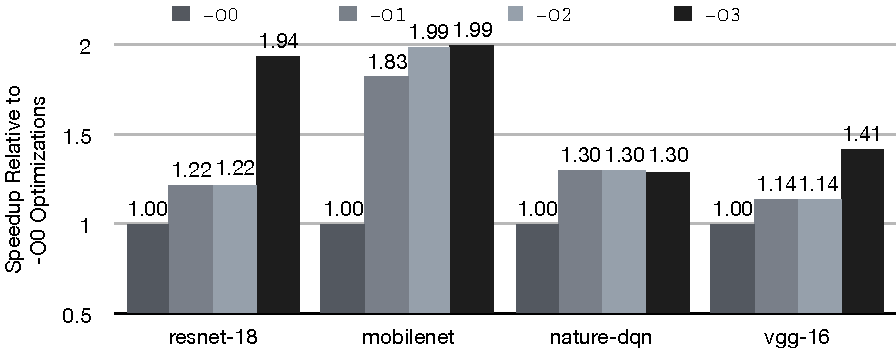
\includegraphics[width=0.5
  %   \textwidth]{fig/eval/optimization_levels.pdf}
  %   \caption{Speedup from increasing the number of graph transformations in \relay (\texttt{-O1}, \texttt{2}, \texttt{3}), relative to no optimizations at all (\texttt{-O0}). We show that, by composing passes, we can monotonically improve performance on vision benchmarks running on the NVIDIA GTX 1080 Ti.}
  %   \label{fig:opt-eval}
  % \end{figure}

  % We demonstrate that \relay can facilitate composable optimizations,
  % by evaluating vision workloads under incremental optimization levels, denoted \texttt{-On}:
  % \begin{itemize}
  %   \item \texttt{-O0} does not apply any program transformation passes.
  % % (it applies a single pass to translate the ``batch norm'' operator into simpler arithmetic
  % % operators but \relay{} has no other implementation of ``batch norm'').
  %   \item \texttt{-O1} applies an operator fusion pass.
  %   \item \texttt{-O2} additionally applies constant folding, using \relay{}'s interpreter to evaluate away operations on constants.
  %   \item \texttt{-O3} additionally applies four more passes:
  %       (1) \texttt{FoldScaleAxis}, which folds scaling operations into the axis options of other operators,
  %       (2) \texttt{AlterOpLayout}, which alternates operator layouts for better cache performance,
  %       (3) \texttt{CanonicalizeOps}, which canonicalizes the ``bias add'' operator in terms of expanding dimensions and broadcasting for further analysis,
  %       (4) \texttt{CommonSubexpElim}, which lifts common subexpressions.
  % \end{itemize}

  % Figure~\ref{fig:opt-eval} shows mean inference speedup relative to
  %   \texttt{-O0} as \relay applies optimizations more aggressively.
  % Average performance improves by up to 2$\times$ when all optimizations are applied.
  % Most networks benefit greatly from operator fusion.
  % Nature-DQN~\cite{dqn} has simple operators, which don't benefit from optimizations
  %   such as layout transform, explaining why its performance doesn't improve beyond \texttt{-O1}.
  % ResNet-18~\cite{resnet} and VGG-16~\cite{vgg} are two dense convolutional neural
  %   networks which benefit from \texttt{-03} optimizations.
  % These networks contain dense \texttt{conv2d} operators that benefit
  %   from the \texttt{AlterOpLayout} pass.
  % Overall, these results show that \relay lets us compose optimizations
  %   in a way that is beneficial to diverse workloads.

  \subsection{\relay Provides Competitive Performance}
  \label{sec:perf-gpu}

  \begin{figure}[h]
    % 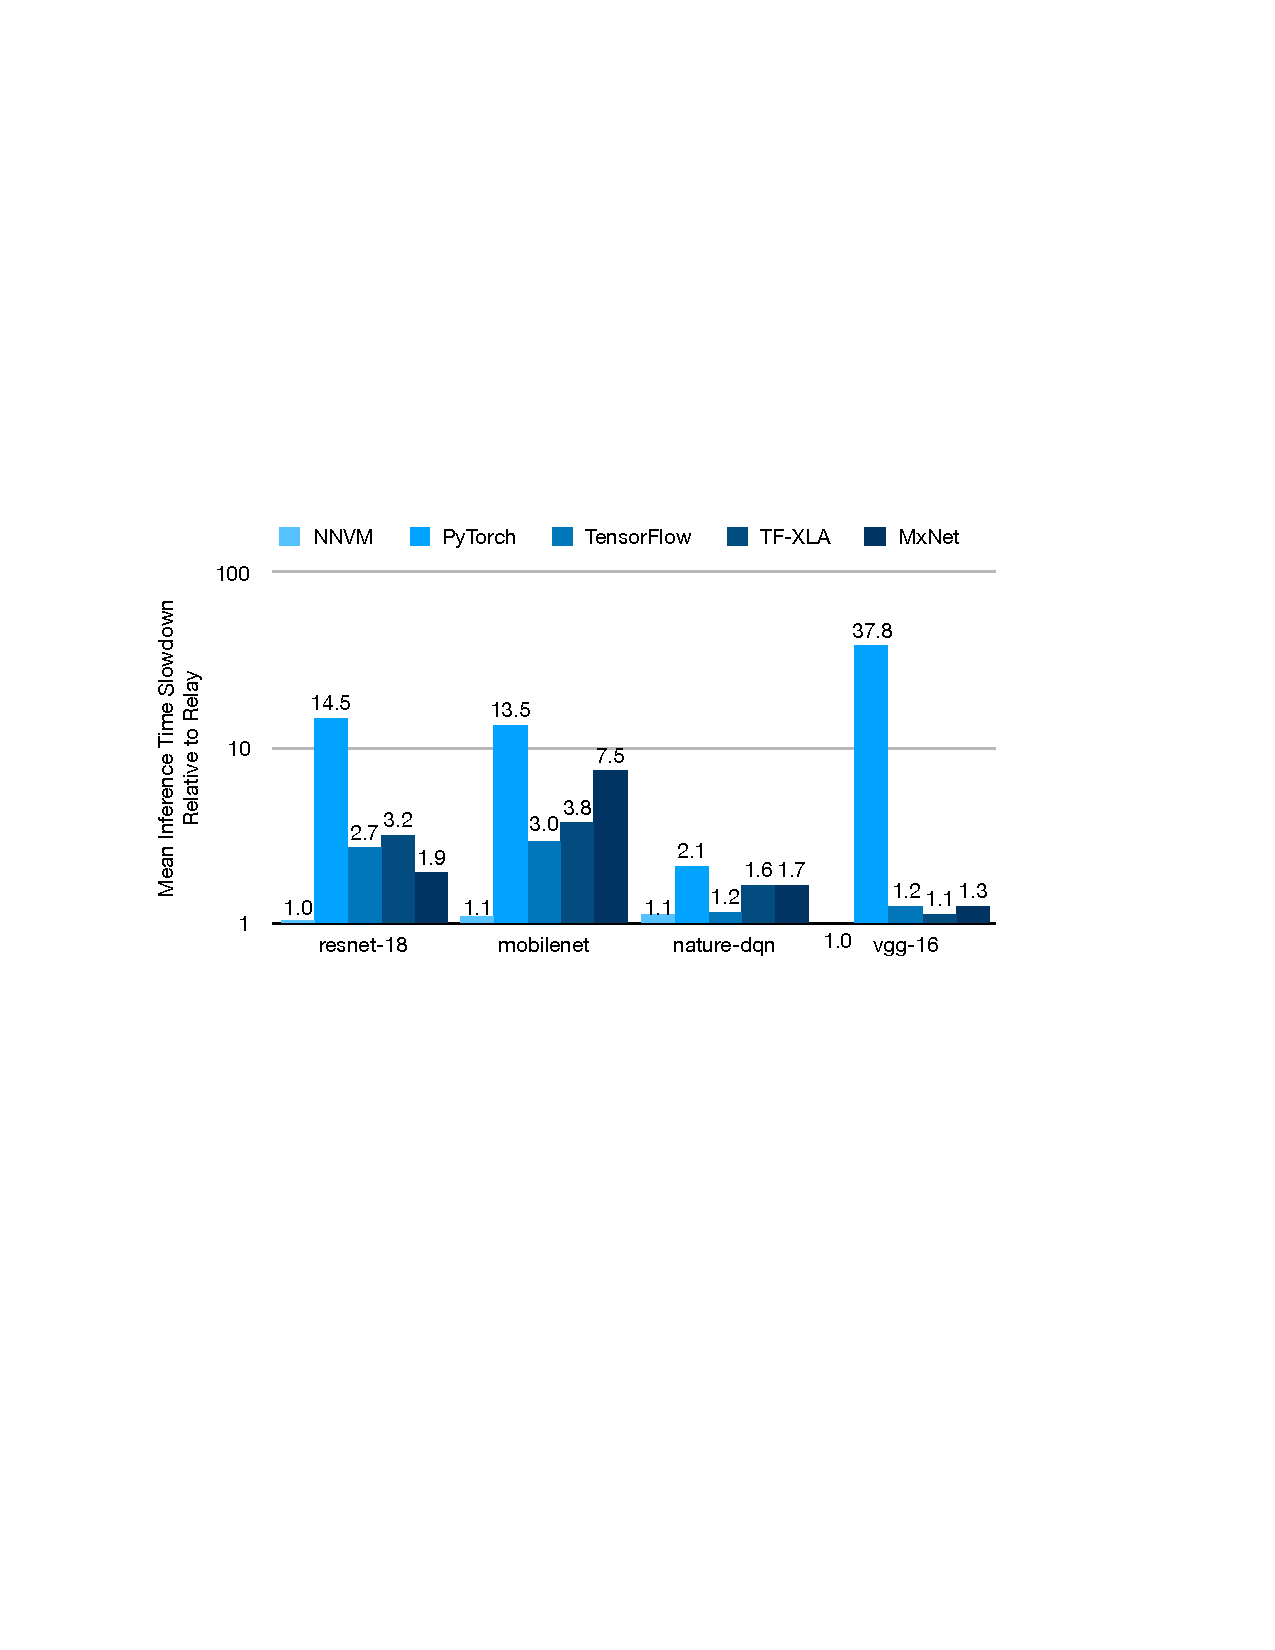
\includegraphics[width=0.6
    % \textwidth]{fig/eval/vision_1080Ti_relay.pdf}
    % \captionof{figure}{
    %   Inference slowdown of popular frameworks relative to \relay on vision
    %     benchmarks running on NVIDIA GTX 1080 Ti GPUs.
    %   \relay provides performance competitive to the state of the art.
    %   We ran 1000 trials for each model and used the AoT compiler.
    % }
    % \label{fig:vision-eval}
  \end{figure}

  \begin{figure}[h]
    % 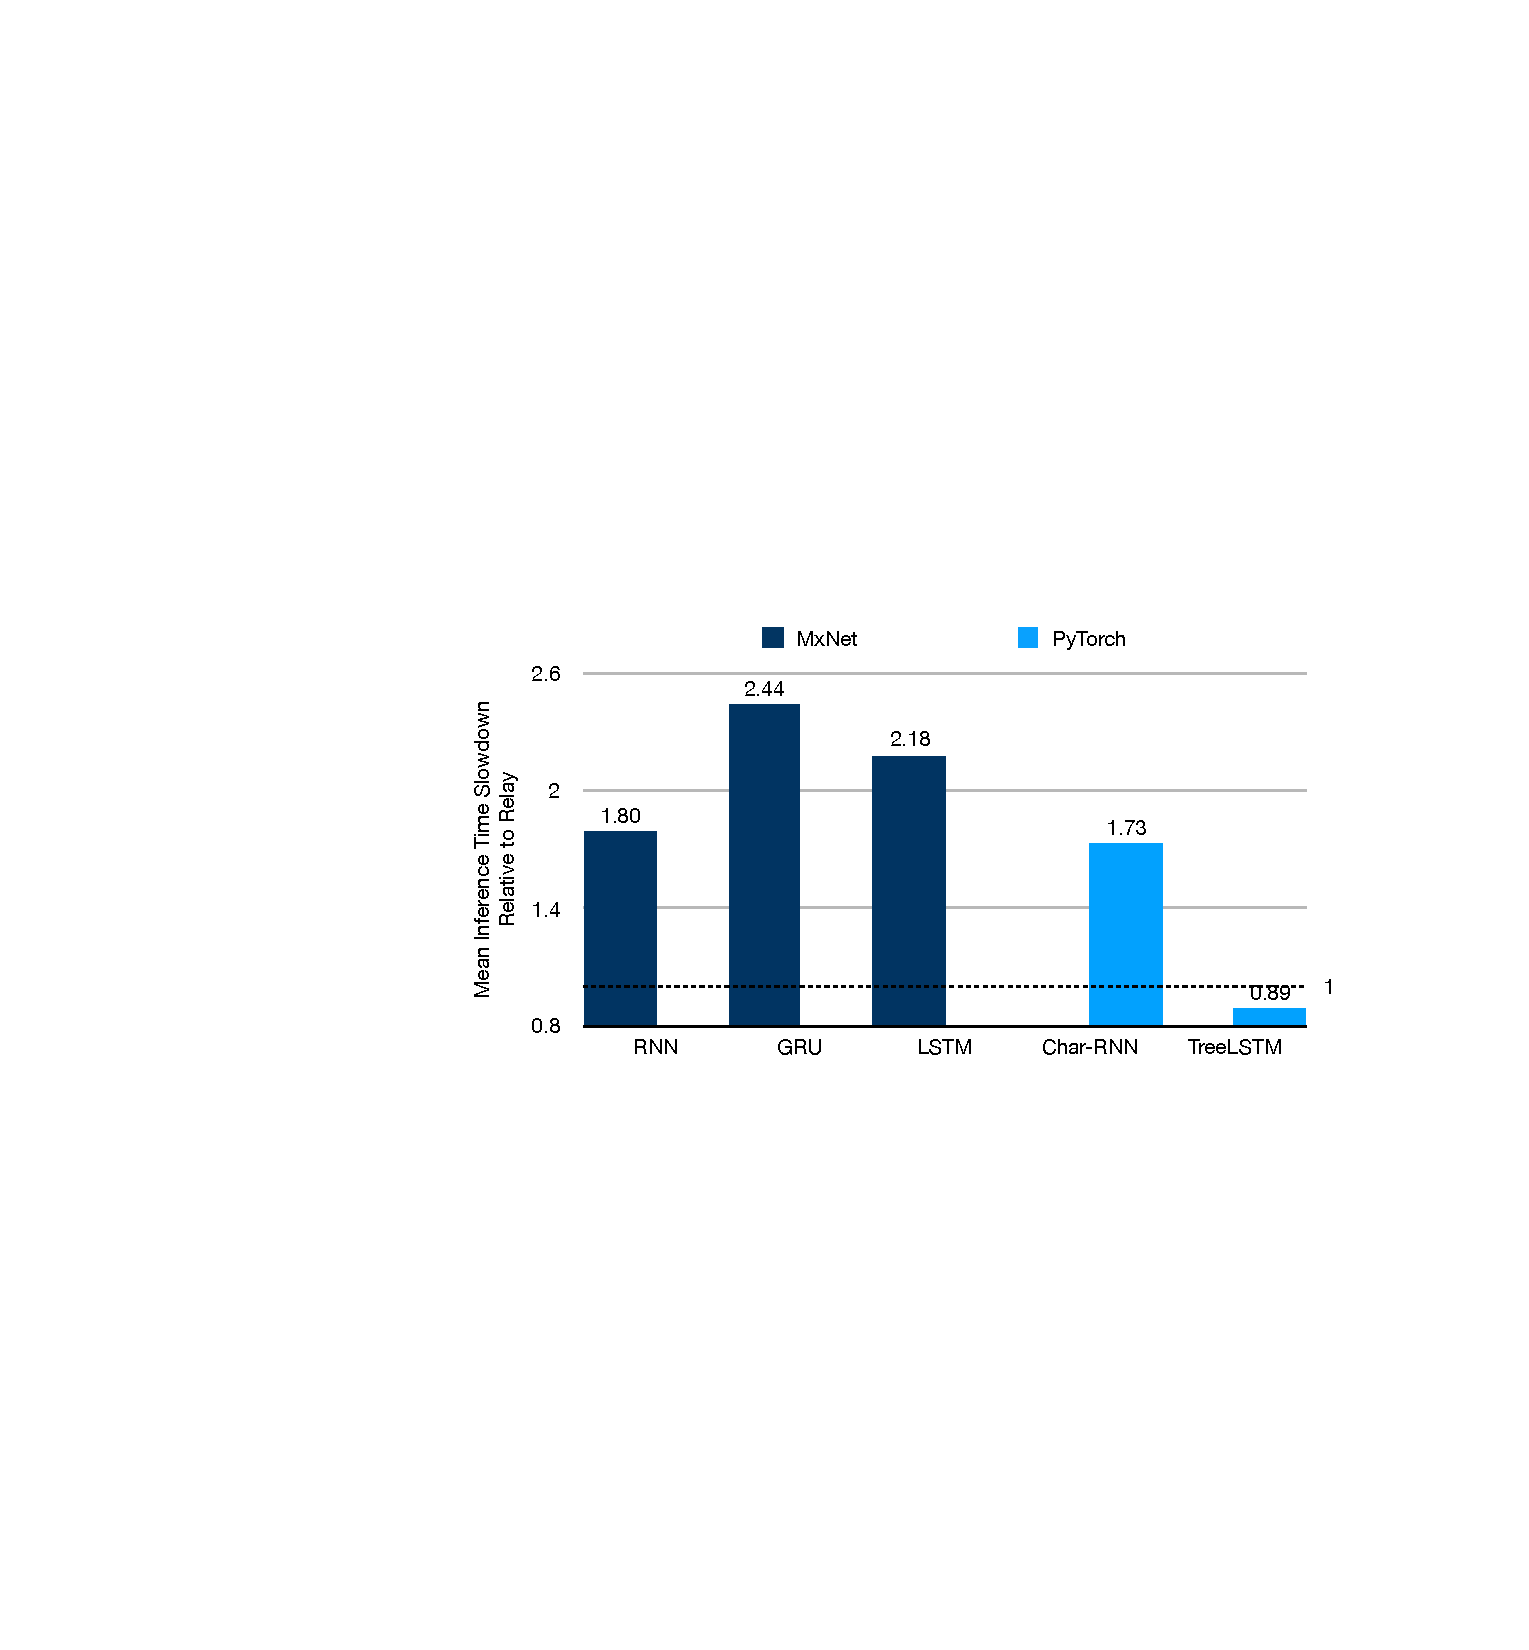
\includegraphics[width=0.6
    % \textwidth]{fig/eval/nlp_TitanV_relay.pdf}
    % \captionof{figure}{
    %   Inference slowdown relative to \relay on NLP benchmarks running on NVIDIA
    %     Titan-V GPUs.
    %   NLP workloads feature control flow,
    %     which makes them more challenging to optimize.
    %   \relay provides performance competitive to state of the art (up to
    %     2.4$\times$ speedup over MxNet on GRU).
    %   We ran 1000 trials for each model, except for CharRNN, on which we used 100 trials.
    % }
    % \label{fig:nlp-eval}
  \end{figure}

  An age-old story in compilers literature is that increasing expressivity
    impacts the global performance of the system.
  We set out to build zero-cost abstractions for \relay,
    governed by Stroustrup's principle, ``What you don't use, you don't pay
    for'' \cite{bjarne}.
  We demonstrate that we can achieve competitive performance on both CPUs and
    GPUs on a wide set of CNNs that are well supported by existing frameworks.
  We evaluated inference time for two classes of workloads: computer vision and natural language processing.
  We compared \relay (using our AoT compiler) to \nnvm,
    TensorFlow, TensorFlow-XLA (Accelerated Linear Algebra), PyTorch, and MxNet.
  We ran the vision and NLP workloads on GTX 1080 Ti and Titan-V GPUs, respectively.

  \paragraph{Vision Evaluation}
  Figure~\ref{fig:vision-eval} compares \relay against state of the art frameworks
    running vision workloads on a GTX 1080 Ti GPU.
  We ran each model with
    batch size 1, a common setting in inference tasks.
  \relay achieves performance on par with \nnvm,
    an existing deep learning graph compiler in use at Amazon.
  \relay outperforms TensorFlow, TensorFlow-XLA, MxNet and
    PyTorch on every benchmark.
  \relay's ability to do aggressive optimizations like operator
    fusion on long chains of operations, generating hardware
    specific implementations, enables it to outperform
    existing frameworks that don't perform inter-operator optimizations.

  \paragraph{NLP Evaluation}
  Figure~\ref{fig:vision-eval} compares \relay against state-of-the-art NLP models on a Titan-V GPU.
  Implementations of the NLP models were not available in all frameworks;
    we used MxNet baselines for RNN, GRU, and LSTM and PyTorch for Char-RNN and TreeLSTM.
  % We ran the models for 1000 iterations per input, except char-RNN, which we ran for 100 ???.
  % To run the RNN, GRU, and LSTM benchmarks in MxNet, and Char-RNN, and TreeLSTM
  %   in PyTorch.
  \relay performs better than MxNet on recursive models
    due to the fact they are implemented in Python using
    MxNet's looping constructs.
  PyTorch instead uses handwritten and heavily optimized
    C implementations of the recursive network cells.
  Due to this we perform slightly \emph{worse} than PyTorch.
  It is interesting to note that our pure \relay
    implementation performs competitively against
    the hand-optimized version.

  \subsection{\relay Handles Challenging Backends}
  \label{sec:low-power}

  \begin{figure}[h]
    % 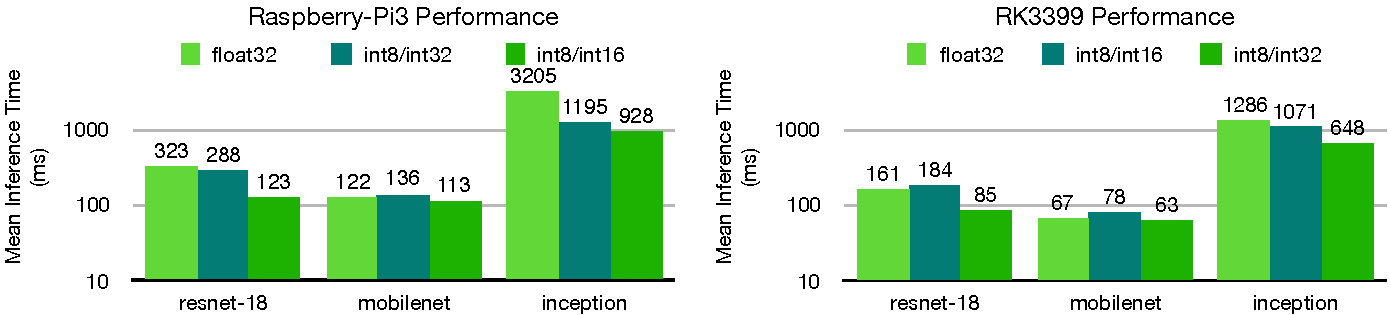
\includegraphics[width=\textwidth]{fig/eval/vision_arm.pdf}
    \caption{
      Inference time (ms) of vision DNNs on low-power platforms using
        different data types.
      \relay allows us to reduce inference time on power-constrained devices by
        easily substituting \texttt{float32} multiplications with \texttt{int8}
        multiplications and \texttt{int16} or \texttt{int32} accumulations (denoted
        at \texttt{int8}/\texttt{int16} and \texttt{int8}/\texttt{int32} respectively).
      We used 1000 trials for each model.
    }
    % \label{fig:arm-eval}
  \end{figure}

  \begin{figure}[h]
    % 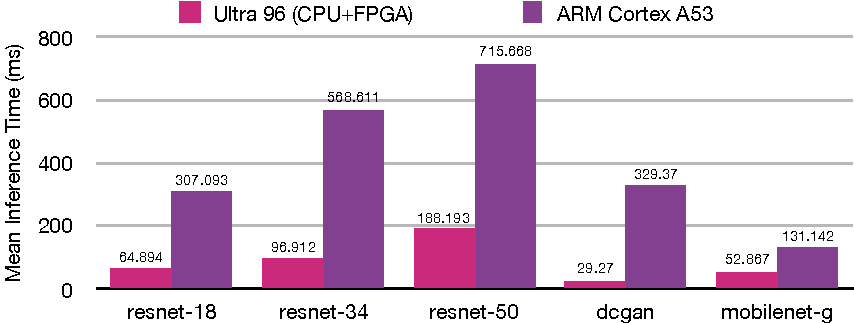
\includegraphics[width=0.6\textwidth]{fig/eval/vision_fpga.pdf}
    \caption{
      Inference time (ms) of vision DNNs on Ultra-96 FPGA-enabled SoC.
      We compare vision workloads that \relay compiles onto the embedded Cortex
        A53 CPU vs. a DNN accelerator implemented on the integrated FPGA fabric.
      Targeting DNN accelerators can unlock up to 11x speedups, but requires a
        multitude of graph-level transformations.
      We used 10 trials for each model.
    }
    % \label{fig:fpga-eval}
  \end{figure}

  \relay can handle challenging scenarios: consider edge inference where energy is a first order
    constraint due to thermal limitations or limited battery life.
  One option is to apply more aggressive quantization: instead of performing expensive
    arithmetic in the floating point domain, simpler and narrower fixed point data is used.
  Another option is hardware acceleration: instead of evaluating
    compute-intensive operations on the CPU, we can offload to a specialized accelerator.

  \paragraph{Quantized Inference on ARM CPUs and GPUs}
  We evaluate the effects of quantized inference applied by \relay on vision workloads running
  on the Raspberry-Pi3 and Firefly RK3399 ARM-based platforms.
  Figure~\ref{fig:arm-eval} shows the effects of different levels
    of quantization applied to low-power devices~\cite{relay_arixv}.
  The numbers show that as we opt for a more aggressive quantization scheme such as \texttt{int8/16} (i.e. 8-bit multiplication and 16-bit accumulation), we achieve much improved performance.

  \paragraph{Targeting Deep Learning Accelerators on FPGAs}
  We evaluated inference time on five models including MobileNet-G \cite{mobilenet}, a grouped variant of the MobileNet architecture; ResNet-18, ResNet-34, and ResNet-50\cite{resnet}; and Deep Convolutional Generative Adversarial Networks \cite{dcgan}, a generative DNN used in unsupervised learning.
  Overall, \relay helps us efficiently offload deep learning operators onto specialized accelerators like VTA.
  Our results in Figure~\ref{fig:fpga-eval} show that we can achieve between 2.5 to 11.7$\times$ reduction in single-batch inference latency by offloading critical operators to the FPGA accelerator.
  These experiments demonstrate \relay's ability to target current and future deep learning architectures:
  \begin{enumerate}
    \item \textit{Heterogeneous FPGA/CPU offloading}: \relay lets us define the rules for offloading specific operators to the FPGA-based accelerator.
    \item \textit{Push-button quantization}: \relay can take a \texttt{fp32} model and convert its parameters to \texttt{int8} in order to enable inference on specialized accelerators.
    \item \textit{Accelerator-friendly data packing:} \relay reorganizes data so it can be effortlessly consumed by a specialized TPU-like accelerator~\cite{tpuv1}.
  \end{enumerate}

\subsection{Tensor VM: Putting the VM in TVM}

We plan to evaluate the VM, by demonstrating in
  static situations that it matches existing
  systems performance, can provide superior performance
  for dynamic networks, and be easily customized
  and extended with new code generation strategies.
My collaborators at Facebook and I will construct
  a new benchmark suite containing dynamic models
  which demonstrate the need for features provided by frameworks
  like PyTorch.
We will extend the PyTorch profiling JIT to better support
  the class of programs \relay can optimize, and make it
  possible for it to use \relay.
Finally we will deeply integrate \relay and PyTorch
   in order to show the combination of dynamic and
   static techniques required.

\subsection{Automatic Tensorization}

We plan to evaluate automatic tensorization by collecting
  a set of ISAs with varying instrinics, semantics,
  datatypes, and bitwidths.
We can use our parametric design \vta to generate a large
  number of designs with varying operations, and semantics.
We have already begun to further parametrize VTA to better
  perform this evaluation.
We then write a description of the primitive operation
  semantics and produce human comparable code
  automatically.
If are able successfully map programs eligible instrinics.



\section{Past Work}
\label{sec:past}

% 3. A description of the work for your dissertation that you have already
% completed and the results you have collected.  Describe the strengths and
% weaknesses of your approach to date, including what it can and cannot do (or
% in the case of results, what those results show and what are the limitations
% of your results).

\subsection{Relay}

Many early DL IR designs made then-convenient design tradeoffs that
  now impede expressing state-of-the-art models and/or
  targeting hardware accelerators.
As a result, frameworks repeatedly
  patch or even fork core framework IRs~\cite{
    tf_fold, tf_lite, tangent, tf_eager, xla, glow, torchscript}.
Such \textit{ad hoc} extensions improve expressivity and
  maintain backwards compatibility with existing execution mechanisms.
However, they are difficult to design, reason about, and implement.
Moreover, the various independently implemented IR modifications are frequently incompatible.

The scenario presented in the introduction demonstrates the three-pronged \textbf{extensibility challenge}
  for DL IRs:
% \begin{enumerate} % [label=\arabic*.]
%   \item \textit{Expressivity}: It should be straightforward to write models involving complex data structures (e.g., trees, graphs, and lists) and control flow.
%   \item \textit{Composability}: It should be straightforward to add and compose new optimizations
%     with existing ones (e.g., quantization, operator fusion, and automatic differentiation).
%   \item \textit{Portability}: It should be straightforward to add new hardware backends
%     (e.g., TPU, Inferentia, and FPGAs)~\cite{tpuv1, inferentia}.
% \end{enumerate}

Previous IRs have struggled to address these challenges because they treat
  each part of the framework as a disconnected set of libraries.
Operators are defined in low-level languages like C++,
  connected with a dataflow graph, and then scripted
  in a host language such as Python;
  analyses cannot traverse the boundaries between these components.
Learning from the steps and missteps of previous IRs, we designed \relay,
  a principled approach to addressing extensibility.
By treating the entire stack as a language
  design problem, \relay enables reasoning across
  abstraction boundaries, which
  improves expressivity, composability, and portability over previous frameworks.
We make the following core contributions:
\begin{itemize}
  \item
  Below we describe \relay, a tensor-oriented, statically typed,
    functional IR.
  Collections of \textit{ad hoc} extensions in previous frameworks
    that patched shortcomings in expressiveness are subsumed by a handful of well-known language
    constructs like let expressions, ADTs, first-class functions, and references.
  In addition to improving expressivity,
    incorporating these features as language constructs
    allows optimizations to more readily compose.
  \item
  By representing DL models as functional programs, we reframe traditional
    DL framework problems as compiler problems.
  Backpropagation becomes a source code transformation,
    transforming an arbitrary \relay function into its gradient function;
    \textit{ad hoc} shape inference becomes principled type inference;
    graph rewriting becomes program optimization;
    and the executor becomes (depending on what the context demands) an
    interpreter, virtual machine, or ahead-of-time compiler.
  Using this correspondence, we adapt existing
    PL techniques to the DL domain.
  \item
    A notable example of this approach is \relay's type system (Section \ref{subsec:type_system}).
    Since operators have complicated semantics, shape inference is usually
      performed when shapes are fully concrete;
      however, at compile time, one does not have that luxury.
    We therefore extend a Hindley-Milner type system with type relations that encode shape
      constraints induced by operators.
    This allows \relay passes to reason about shape information at compile time.
  \item To provide portability,
    we define a platform-agnostic operator language
    and a compiler pass manager, which facilitates the development of
    passes that transform the IR to target new hardware backends.
\end{itemize}

\relay is an open source component of the \tvm project.
It has been deployed at Amazon Web Services, Facebook, Huawei,
  and is currently being adopted by teams at ARM and Qualcomm.
It is used to deploy efficient machine learning to
  both commodity and custom hardware with minimal
  engineering effort.

\subsection{Compiler Framework}
  The \relay pipeline can be split into three classic components:
    the frontend, where input formats are translated to \relay;
    the compiler, which type checks \relay ASTs, applies optimizations,
      and compiles operators;
    and the backend, where an execution mechanism is selected and
      available hardware accelerators are utilized.

  \subsection{Frontend}

  There are several ways to write an \relay program.
  A user can build an in-memory representation of
    a program in C++ or Python;
    parse one written in the \relay text format;
    or load one from the on-disk serialization format,
    similar in design to LLVM's bitcode.
  Models from popular frameworks, including
    TensorFlow, PyTorch, MxNet, Keras, and DarkNet, as well as interchange
    formats, such as ONNX, may be imported directly into \relay.
  \subsection{Compiler}
  Once an \relay abstract syntax tree (AST) is produced,
    the program is optimized by applying a series of \relay-to-\relay
    passes.
  Between each pass, \relay performs type inference and checking,
    rejecting malformed programs as well as populating shape and type
    information that passes can utilize.
  \relay optimizations consist of both traditional compiler
    optimizations as well as domain-specific optimizations.
  Traditional compiler optimizations include constant folding,
    common subexpression elimination,
    and dead code elimination.
  DL-specific optimizations include
    operator fusion,
    quantization,
    layout transformation,
    and accelerator-specific optimizations.

  \relay produces machine-specific code
    by decomposing the problem of code generation into multiple distinct phases.
  % See Figure~\ref{fig:pipeline} for a visual overview of each stage.
  Since \relay is a high-level IR, it depends on a low-level code generator,
    such as \tvm or Halide,
    to produce dense linear algebra kernels~\cite{tvm_osdi18, halide}.
  We use \tvm in our experiments.
  Low-level kernel compilers focus on generating highly efficient operators.
  The generated kernels have a fixed calling convention and do not
    handle allocation. Instead, they expect inputs and outputs to be preallocated.
  From an optimized AST,
    the compiler extracts a set of \relay operators,
    translates them to TVM expressions,
    and then compiles to available hardware targets.
  The resulting output is an
    object file that contains the compiled operators
    and an \relay program that invokes these primitives.
  In our prototype implementation,
    we are able to target CPU, GPU,
    iOS and Android mobile devices,
    custom accelerators, and FPGAs.

  \subsection{Backends}
  After primitive operators are lowered,
    the remaining \relay program is the glue that ties
    together operator invocations, allocation, control-flow,
    recursion, and high-level data structures.
  There are multiple options for executing the combined full program:
      the \relay interpreter (with JIT compilation),
      the \tvm graph runtime,
      and an ahead-of-time compiler
      that converts programs to C++.

  \subsection{IR}
  % \begin{figure}[!t]
%     \begin{jmpgrammar}
%       \bnfrule{REAL}{\real} \is{\mathbb{R}}\\
%       \bnfrule{NAT}{\nat} \is{\mathbb{N}}\\
%       \bnfrule{NAME}{\rName} \is{\texttt{(}\text{`\_'}\inlineAlt[a-zA-Z]\texttt{)}\ \
%       \atLeastZero{\text{`\_'}\inlineAlt[a-zA-Z]\inlineAlt[0-9]}}\\
%       \bnfrule{TYPE NAME}{\typename} \is{[A-Z]\ \ \atLeastZero{\text{`\_'}\inlineAlt[a-zA-Z]\inlineAlt[0-9]}}\\
%       \bnfrule{GLOBAL VAR}{\gvar} \is{\kwd{@}\rName}\\
%       \bnfrule{LOCAL VAR}{\lvar} \is{\kwd{\%} \rName}\\
%       \bnfrule{GRAPH VAR}{\graphVar} \is{\kwd{\%} \nat}\\
%       \bnfrule{TYPE VAR}{\tyvar} \is{\rName}\\
%       \bnfrule{OPERATOR}{\op} \is{\rName}\\\\
%       \bnfrule{Program}{\program} \is{\atLeastOne{\defn\inlineAlt\typedef}}
%         \alt{\expr}\\\\
%       \bnfrule{Param}{\param} \is{\rParamRule}\\
%       \bnfrule{Type Param}{\tyParam} \is{\rTyParamRule}\\\\
%       \bnfrule{Definition}{\defn} \is{\rDefnRule}\\\\
%       \bnfrule{Type Definition}{\typedef} \is{\rTypeDefRule}\\\\
%       \bnfrule{Kind}{\kind} \is{\kwd{BaseType}}
%         \alt{\kwd{Shape}}
%         \alt{\kwd{Relation}}
%         \alt{\kwd{ADT}}
%         \alt{\kwd{Type}}\\\\
%       \bnfrule{BaseType}{\basetype} \is{\kwd{int} \nat \maybe{\kwd{x} \nat}}
%         \alt{\kwd{float} \nat \maybe{\kwd{x} \nat}}
%         \alt{\kwd{bool} \maybe{\nat}}\\\\
%       \bnfrule{Shape}{\shape} \is{\kwd{(} \seq{\nat} \kwd{)}}\\\\
%       \bnfrule{Pattern}{\patt} \is[constructor]{\op \kwd{(} \seq{\patt} \kwd{)}}
%         \alt[wildcard]{\wildcard}
%         \alt[variable]{\lvar\ \maybe{\typeanno}}
%     \end{jmpgrammar}
%   \end{figure}
  \begin{figure}[t]
    % \ContinuedFloat
    \begin{jmpgrammar}
      \bnfrule{Expr}{\expr} \is[local var]{\lvar}
        \alt[global variable]{\gvar}
        \alt[constant tensor]{\kwd{const} \kwd{(} \texttt{(}\real\inlineAlt\bool\texttt{)} \kwd{,} \shape \kwd{,} \basetype \kwd{)}}
        \alt[call]{\expr \maybe{\tyargs} \args\vspace{0.2em}}
        \alt[let]{\rLetRule}
        \alt[\kwd{let}\ \kwd{\%}\_\ \kwd{=}\ \expr\kwd{;}\ \expr]{\rAnonLetRule}
        \alt[graph let]{\rGraphLetRule}
        \altSpace{0.5em}{function}{\rFnRule}
        % \altSpace{1em}{type cast?}{\kwd{(} \type \kwd{)} \expr}
        \altSpace{1em}{tuple formation}{\rTupRule}
        \alt[tuple proj.]{\rTupProjRule}
        \alt[if-else]{\rIfElse{\expr}{\expr}{\expr}}
        \altSpace{0.5em}{pattern match}{\rMatchRule}
        \altSpace{1em}{operator}{\op}
        % TODO: When will we have gradient as a first-class operator?
        % \alt[gradient]{\kwd{grad}\kwd{(}\expr\kwd{)}}
        \alt[new ref]{\kwd{ref}\kwd{(}\expr\kwd{)}}
        \alt[get ref]{\kwd{!} \expr}
        \alt[set ref]{\expr \kwd{:=} \expr}\\\\
      \bnfrule{Type}{\type} \is[base type]{\basetype}
        \alt[shape]{\shape}
        \alt[tensor type]{\kwd{Tensor} \kwd{[} \shape \kwd{,} \basetype \kwd{]}}
        \alt[type variable]{\tyvar}
        \alt[function type]{
          \begin{split}
          \kwd{fn}\ &\rTyParamsRule\\
          &\kwd{(} \seq{\type} \kwd{)}\ \rettype\\
          &\maybe{\relations}
          \end{split}
          }
        \alt[ref type]{\kwd{Ref} \kwd{[} \type \kwd{]}}
        \alt[tuple type]{\kwd{(} \seq{\type} \kwd{)}}
        \alt[type call]{\type \kwd{[} \seq{\type} \kwd{]}}
        \alt[type name]{\typename}
    \end{jmpgrammar}
    \caption{\textmd{The BNF Grammar for the \relay{} language.}}
    \label{fig:short_bnf}
  \end{figure}


  The \relay IR is a high-level, functional, differentiable language.
  One can understand \relay by starting from a subset of \relay
    that represents an idealized computation graph IR and
    incrementally growing to the full \relay IR.
  A computation graph, in its simplest presentation, is a directed acyclic
    graph with multiple inputs and a single output.
  The syntax of an equivalent computation graph is realized by
    a language with three rules (1) \verb|variable|s, (2) function \verb|call|s,
    and (3) \verb|operator|s, see Figure~\ref{fig:short_bnf} for the corresponding rules.

  \subsection{Multi-Output}

  This subset lacks useful features that are present in IRs used
    in practice.
  For example, common operators such as \verb|split|, which splits
    a tensor along a particular axis, require multiple outputs.
  In order to handle these programs,
    computation graph IRs have added primitive support
    for multiple outputs.
  Multiple outputs can be modeled as tuples, which can
    be added with just two rules (1) \verb|tuple formation|
    and (2) \verb|tuple projection|.

  \subsection{Let}

  By construction, computation graphs enjoy implicit sharing of subcomputations via multiple outgoing
  dependency edges.
  Implicit sharing is useful for both execution and analysis,
    because it enables users to uniquely identify subgraphs.
  Previous frameworks often obtain sharing by using a host
    language's name binding to construct a graph.
  General purpose programming languages, on the other hand, provide \textit{explicit}
    sharing via binding constructs, such as \verb|let|.
  In programs free of scope, ordering, and effects, implicit sharing
    and explicit sharing are semantically equivalent.
  However, in the presence of these three, implicit sharing does not adequately preserve the semantics
    of effects, since their ordering is not well-defined.
  Since user programs contain scope, ordering, and effects in practice,
    previous systems have been forced to provide workarounds.

  For example, TensorFlow's eager mode inserts dummy control edges
    in its generated graphs to impose an ordering on effects.
  The lack of lexical scope in traditional graphs complicates language features
    such as first-class functions and control-flow~\cite{funarg, funarg_sol}.
  The lack of explicit scoping information also weakens the ability
    to provide precise versions of traditional analyses, such as liveness.
  The addition of a humble \verb|let| binding, well studied in programming languages,
    enables explicit sharing and provides an elegant solution to the problems outlined above.

  \subsection{Control Flow}

  \begin{figure}[htb!]
    \begin{tabular}{ccc}
    \begin{minipage}{0.5\textwidth}
    \begin{minted}[fontsize=\small]{python}
  i = tf.constant(1)
  j = tf.constant(1)
  k = tf.constant(5)

  def c(i, j, k):
    return
      tf.equal(
        tf.not_equal(
          tf.less(i + j, 10),
          tf.less(j * k, 100)),
         tf.greater_equal(k, i + j))

  def b(i, j, k): return [i+j, j+k, k+1]

  tf.while_loop(c, b, loop_vars=[i, j, k])
    \end{minted}
    \end{minipage}
  & \hspace{-3.0em}
  \begin{Huge}
    $\Rightarrow$
  \end{Huge}
  &
    \begin{minipage}{0.5\textwidth}
    \begin{minted}[fontsize=\footnotesize]{python}
  let %while_loop =
    fn (%loop_var0: Tensor[(1,), int32],
        %loop_var1: Tensor[(1,), int32],
        %loop_var2: Tensor[(1,), int32]) {
      %0 = add(%loop_var0, %loop_var1)
      %1 = less(%0, meta[Constant][0])
      %2 = multiply(%loop_var1, %loop_var2)
      %3 = less(%2, meta[Constant][1])
      %4 = not_equal(%1, %3)
      %5 = add(%loop_var0, %loop_var1)
      %6 = greater_equal(%loop_var2, %5)
      if (min(equal(%4, %6))) {
        %9 = add(%loop_var0, %loop_var1)
        %10 = add(%loop_var1, %loop_var2)
        %11 = add(%loop_var2, meta[Constant][2])
        %while_loop(%9, %10, %11)
      } else {
        (%loop_var0, %loop_var1, %loop_var2)
      }
    }
  %while_loop(meta[Constant][3],
              meta[Constant][4],
              meta[Constant][5])
    \end{minted}
    \end{minipage}
    \end{tabular}
    \caption{
      A simple TensorFlow loop in the user-facing DSL and the \relay
        loop produced by automatically converting it.
      Note the TensorFlow while loop corresponds neatly to a tail recursive
        function.
      The \relay text format supports a ``metadata'' section which functions
        as a constant pool among other things.
      \texttt{meta[Constant][n]} represents the \texttt{n}-th constant in the
        pool.
    }
    \label{fig:tf_to_relay_loop}
    \end{figure}

  Neural networks increasingly rely on control flow, forcing frameworks based on computation graph IRs
  to support this construct; however, control flow extensions are generally \textit{ad hoc}.
  Even in the presence of control flow-free models, looping
    constructs are necessary to implement optimization algorithms
    such as SGD.
  Furthermore emerging architectures are beginning to make greater use of
     control flow, with many architectures exposing custom control
     combinators such as loops, maps, folds, and scans.
  The central challenge is a flexible and extensible encoding of
    control flow operations.
  The functional programming community has demonstrated recursion and pattern matching are sufficient
    to implement arbitrary combinators for control flow and iteration.
  To support the definition of functional loops we enrich \relay with two more language
    features to implement arbitrary combinators: \verb|if| and first-class recursive functions.
  The guard expression in \relay's \verb|if| expression operates over rank-0 boolean tensors,
    which represent booleans.

  \subsection{First-Class Functions}

  A computation graph is a single expression
    from multiple inputs (i.e. its free variables) to multiple outputs.
  While it may be tempting to reinterpret a graph as a function, it lacks functional abstraction
    and named recursion.
  Adding the ability to name functions and pass them as first-class values dramatically increases
    \relay's expressivity, allowing it to encode generic
    higher-order functions and readily use techniques used in functional
    compilers like automatic deforestation.
  First-class functions enable passes such as
    automatic differentiation, and simplify
    the framework importers which map higher-level programs to our IR~\cite{myia}.
  For example, an instance of TensorFlow's looping construct \verb|tf.while_loop|
    can be represented as a single specialized loop function
    or a generic fold over the full loop state.
  See Figure~\ref{fig:tf_to_relay_loop} for an example of this conversion (via
    the \relay TensorFlow frontend).

  \subsection{Data Abstraction}
  Earlier, we extended the language with tuples to
    emulate behavior of existing IRs.
  Deep networks require additional data types like lists,
    trees, and graphs~\cite{char-rnn, tree_lstm, graph_lstm}.
  \relay borrows a generic and principled way to
    extend a language with new data types:
    algebraic data types (ADTs).
  To support them we add (1) a type declaration mechanism and
    (2) pattern matching.
  One may question why \relay has \verb|if| when it could be subsumed by \verb|match|:
    \verb|if| is still necessary because tensors are primitives, not ADTs.
    % and thus do not have a recursion principle that characterizes their match behavior.

  The resulting language is a familiar strict functional language,
    resembling the core of languages like OCaml and SML.
  Our language makes domain-specific deviations from existing work,
    and we have provided a full listing
    of its syntax, operational semantics, and type rules
    in the appendix.
  A functional language provides a few notable advantages.
  Its pure fragment represents idealized computation graphs free
    from effects. This fragment can be easily optimized by end users who
    can reason about it as pure dataflow.
  For this reason, \relay is pure by default but exposes a limited
    form of mutation via ML-style references that we have
    primarily used for automatic differentiation.

  \relay is more expressive than many previous frameworks and this expressivity introduces new challenges.
    Previous essential functionality such
     as shape inference and automatic differentiation must be adapted for
     our new IR.
  How does one reason about the shapes of operators when the input is unknown?
  How does one backpropagate over pattern-matching, control, data types, and mutation?
  In the following subsection we demonstrate how one can adapt techniques
    from type inference and checking to \relay.

  \subsection{Type System}
  \label{subsec:type_system}

  Computation graph IRs rely on typing in the form of
    datatype and shape inference.
  Datatype and shape inference is the process of computing the
    concrete datatypes (e.g., \verb|float32|, \verb|int32|) and shapes (e.g., $(10, 5)$, $(100, 1, 32)$) of all
    tensors in a computation graph.
  Deep learning frameworks and compilers use static shape information
    to perform allocation, check correctness, and facilitate optimization.
  Precise static shape information is also valuable for traditional loop
    optimizations, data layout transformations, tensorization, and
    optimizations that are necessary to map to hardware accelerators' unique ISAs.

  Shape inference is usually formulated as a simple analysis over the dataflow graph that
    propagates shape information.
  Shape inference looks remarkably similar to type inference.
  Unlike type inference, though, shape inference is separate from the type system and
    does not provide types for functions or data structures.
  Handling shape inference at compile time is desirable, because it allows optimizations to take
    advantage of this information even though certain shapes may be symbolic. Can shape information be encoded in static types?
  % If we type \relay as simply typed lambda calculus,
  %   we gain a simple system, but one that can not represent polymorphism,
  %   and lacks shape information.
  % Even with the addition of polymorphism, there is no representation of static
  %   shape information.
  It is possible to model arbitrarily complex static properties, such
    as shape information, with dependent type theory, but such
    a design incurs significant user complexity.
  % Adopting a well known type system allows the application of
  %   classic techniques, but standard type systems do not
  %   provide a solution for tracking static shape information.
  \relay's type system is designed to balance the desire for static tensor shapes
    without limiting the language's expressiveness.
  In this subsection we describe how to extend a polymorphic type system with shape
    information and type inference with shape inference.

  \begin{figure}
    \begin{footnotesize}
      \judgbox{\typecheck{\typeCtx}{\varCtx}{\expr}{\type}}{Expression $\expr$ has type $\type$ in type context $\typeCtx$ and variable context $\varCtx$.}
      \begin{inference}
      \jmpInfer{Relation-T}
         {\Delta, T_1 : \texttt{Type}, \ldots, T_n : \texttt{Type} \vdash (Rel(T_1, T_2, \ldots, T_n) \in \{ \top, \bot \}) }
         {\typecheck{\typeCtx}{\varCtx}{Rel}{\texttt{Relation}}}

      \jmpInfer{Type-Func-Def}
        {\forall{i \in [1, r]} \, \Delta; \Gamma \vdash R_i(T_1, \ldots, T_n, O) \\
         \Delta; \Gamma, a_1 : T_1, \ldots, a_n : T_n, \\
         f : \kwd{fn}( T_1, \ldots, T_n) \rightarrow O \kwd{ where } R_1, \ldots, R_r \vdash body : O}
          {\Delta; \Gamma \vdash \kwd{def @} f\kwd{(}a_1\kwd{:} T_1\kwd{,} \ldots
          a_n\kwd{:} T_n\kwd{)} \rightarrow O \kwd{ where } R_1, \ldots, R_r \kwd{ \{ } body \kwd{ \}} : \\
          \kwd{fn}(T_1, \ldots, T_n) \rightarrow O \kwd{ where } R_1, \ldots, R_r }

      \jmpInfer{Type-Call}
         {\Delta; \Gamma \vdash f : \kwd{fn} (T_1 \kwd{,} \ldots \kwd{,} T_n) \rightarrow O
           \kwd{ where } R_1, \ldots, R_r
           \\ \Delta; \Gamma \vdash a_1 : T_1, \ldots, a_n : T_n
           \\ \forall{i \in [1, r]} \, \Delta; \Gamma \vdash R_i(T_1, \ldots, T_n, O)}
         {\typecheck{\typeCtx}{\varCtx}{f(a_1, \ldots, a_n)}{O}}
      \end{inference}
    \end{footnotesize}
    \caption{Examples of \relay's typing inference rules, namely the rules for function definitions and function calls,
      where $\Delta$ is the environment for types and $\Gamma$ is the environment for variables. These demonstrate
      that type relations must hold at each call site.}
    \label{fig:partial-inference-rules}
  \end{figure}

  \subsection{Tensor Types}

  The primitive value in \relay is a tensor, which has
    type $Tensor[s, bt]$ where $s$ is a shape and $bt$ is a base type.
  Elements of base type are floating point numbers and
    integers of specific bit widths and number of lanes.
  This design decision is inspired by LLVM,
    which supports arbitrary-width integer types.
  The parameterization by lanes helps represent vectorized data types, which are supported
    by many CPUs and hardware accelerators.
  To ensure \relay can offload tensor computation to devices
    with greatly varying architectures,
    \relay's kinding rules only permit tensors to contain
    base types, preventing, for example, tensors of closures.

  The shape of a tensor is a tuple of integers describing the tensor's dimensions.
  In general, these dimensions may depend on arguments to an operator.
  A dimension may be a variable or arithmetic expression that indicates how the
    output shape of an operator depends on those of its inputs.
  Functions may be polymorphic over shapes, which results
    in shape constraints that must be solved during type inference.
  Sec.~\ref{sec:inference} describes the process.
  \relay also supports a special shape called \verb|Any|, which is used
    to indicate that we do not have static shape information about a particular dimension.

  \subsection{Operators and Type Relations}

  A difference between general purpose programming models and those tailored to deep learning
    is the use of operators as the primitive unit of computation.
  The ability to add new operations to \relay requires a type system that can adapt to
    complex shape relationships between input and output types.
  Many operators have types that can be defined
    as functions of the input types.
  Unfortunately some are not only functions,
    but also relations that specify constraints between input and output shapes.
  A key extension of \relay over traditional type systems is the addition of type relations
    to express these constraints.
  When developers add a new operator to \relay, they may constrain its
    type with existing relations or add their own.
  Function types (including those of operators) may include
    one or more type relations over an arbitrary subset of the argument types and the return type.
  The type checker enforces that these relationships hold at the call site.
  These relations may be viewed as a verification condition induced at a
    function call site, where the formula is a conjunction of the relations.
  For example, primitive operators are assigned types that are universally quantified over
    both the input and output types.
  We can then use a type relation to encode a constraint that must hold later
    when type checking observes specific input and output types.
  Type relations are opaque in the \relay IR: they are implemented in the
    meta-language and registered when defining an operator.
  However, they may be reused across different implementations.
  For example, we use a relation that describes the
    broadcasting rule for all elementwise operations.

  \subsection{Type Inference}
  \label{sec:inference}

  The most interesting parts of the type system
    are where shape computation occurs.
  We highlight a few examples of \relay's inference
    rules in Fig.~\ref{fig:partial-inference-rules};
    the full typing rules can be found in the appendix.
  In this subsection we focus on design decisions behind \relay's type system
    and the implementation of type inference.
  To incorporate type relations into \relay's type system, we enrich
    a Hindley-Milner type inference algorithm with
    a constraint solver for type relations.
  \relay's inference algorithm has three steps: first it
    performs a pass over the AST generating types (potentially involving type variables)
    as well as populating the set of relations,
    then it solves the incurred constraints,
    and finally it assigns types to each expression in the AST.
  A type relation is implemented as a function in the
    meta-language and represents the symbolic relations between
    the input and output types of an object-language function.
  When the type inference algorithm visits a function call site, the function's type relations are
    instantiated to the types at the call site and added to a queue of relations waiting to be
    solved.
  The relationships between the call's type variables and its relations are are added to a
    bipartite undirected dependency graph where the two disjoint sets are type variables and type relations.
  Traditional unification constraints are represented using a modified union-find structure that
    integrates with the dependency graph.

  Once the queue is populated, the algorithm will dequeue a relation and attempt to solve it.
  There are two cases when solving a type relation:
  \begin{enumerate}
    \item If all the relation's type variables
    are concrete, we call the type relation function. If that function returns true, the
    constraint is discharged. Otherwise, type checking fails.
    \item If any type is fully or partially symbolic, the
      algorithm will propagate
      existing concrete type information via unification.
    All relations affected by new assignments to type
      variables (as determined by the dependency graph)
      are moved to the beginning of the queue.
    If the current type relation is now completely solved, we
    discard it to avoid unnecessarily visiting it again.
  \end{enumerate}

  Our fine-grained dependence graph provides the transitive dependencies
    between relations and unification variables.
  The use of fine-grained dependencies enables our algorithm to
    only retry a minimal number of relations when we
    learn a new variable assignment.
  We run this to fixpoint or until the queue is empty.
  If the queue is not empty and no progress is made between iterations,
    then at least one variable is under constrained and inference fails.
  Note that a type relation's implementation can
    compromise type soundness, as they are axiomatic descriptions
    of operations implemented outside of \relay.
  Luckily, in practice, the number of type relations needed to express most of \relay's
    operators is relatively small, and their implementations are generally straightforward
    and amenable to exhaustive testing.
The above sections discuss the core of \relay, a full-length paper under submission\cite{relay_arixv}
  details its design and implementation.
